% !TEX root = omar-thesis-proposal.tex
%\section{Proposed Contributions}\label{contributions}
%We seek to introduce language-integrated mechanisms that permit library-based implementations of features that compare to and  go beyond the features built into modern programming systems. However, we seek to avoid the associated {metatheoretic} issues and  maintain the ability to understand and reason about libraries modularly, and by a type-based discipline. %This is accomplished by organizing extension logic around types and scoping it to or around expressions of the type it is associated with, rather than applying it globally or within an explicitly delimited scope as in previous mechanisms. 

% To motivate our approach, let us return to our example of regular expressions. We observe that every feature described in Sec. \ref{regex} relates specifically to how terms classified by a type for regular expression patterns, e.g. \verb|Pattern|, should behave. Feature 1 calls for specialized syntax for its introductory form. Features 2a and 2b relate to which operations on patterns exist and how they should be typechecked. Feature 3 discusses editor services only relevant when editing a term of such a type. Feature 2c relates to the semantics of a related  type constructor classifying strings known to be in a regular language.% type that the logic in Sec. \ref{regex}  needs to be considered. 

% Indeed, this is a common pattern: the semantics of programming languages (and logics) have long been organized around their types (equivalently, their propositions). %One of the principal tasks of the logical analysis of a given proposition is to find out the method of verification for that proposition.
% For example, Carnap in his 1935 book \emph{Philosophy and Logical Syntax} stated \cite{carnap1935philosophy}:
% \begin{quote}
% One of the principal tasks of the logical analysis of a given proposition is to find out the method of verification for that proposition.
% \end{quote}
% In two modern textbooks about programming languages, \emph{TAPL} \cite{tapl} and \emph{PFPL} \cite{pfpl}, most chapters describe the syntax, semantics and metatheory of a new type constructor and its associated  operators (collectively, a \emph{fragment}) in isolation. Combining the fragments from different chapters into complete languages is, however, a language-external (that is, metamathematical) operation. In \emph{PFPL}, for example,  the notation $\mathcal{L}$\{$\rightarrow$ \verb|nat| \verb|dyn|\} represents a language that combines the arrow ($\rightarrow$), \verb|nat| and \verb|dyn| type constructors\footnote{We can consider base types like $\mathtt{nat}$ and $\mathtt{dyn}$ as being trivially indexed type constructors, see Sec. \ref{att}.} and their associated operators. Each of these are defined in separate chapters, and it is generally left unstated that the semantics developed separately can be combined conservatively, i.e. with all the fundamental metatheory left intact, a notion we will refine later. This is intuitively justified by a sense that the rules in each chapter seem ``well-behaved'' in that they  avoid violating the autonomy of other fragments. %This organization has long been employed in the study of logic as well. 
% For example, they do not introduce a new value of a type defined in another fragment, because this would render invalid any conclusions arrived at by induction over value forms for that type. 

% If we can somehow formalize this notion of a ``fragment'' and ``autonomy'' and internalize it into the language itself, rather than leaving it as a ``design pattern'' that only informally guides the work of a central language (or textbook) designer, we might achieve  a safely extensible language, i.e. one where separately defined embeddings of  fragments as libraries can be safely combined. Doing so without limiting expressiveness or weakening the system's metatheory is precisely the topic of this thesis. %e of organizing a fragment around the type constructors it introduces, and
% %We call a type constructor defining new syntax, semantics or editor services an \emph{active type constructor}. %This choice, of associating extensions with type constructors rather than term constructors, avoids many issues collectively associated with the \emph{expression problem}, as we will discuss later.


%As we will show, taking a type-oriented point-of-view provides a means to satisfy this principle.
%Making this precise and showing how the language can preclude poorly-behaved fragments from causing problems, while retaining the ability to define interesting fragments, is the focus of this thesis.

%But enforce a golden rule: that each builder of a logic respects every other's autonomy. % That is our goal in this thesis. %By constraining the extension logic itself by various means we will show that the system as a whole can also maintain many other important safety and non-interference properties that have not previously been achieved. 
%We call types with such logic associated with them \emph{active types} and systems that support them \emph{actively-typed programming systems}. 

%\subsection{Proposed Contributions}
% The goal of the research being proposed here is to design \emph{language-integrated extension mechanisms} that give providers the ability to define, within libraries, new features like those above that have previously required central planning, 
% %\footnote{One might compare today's programming systems to  {centrally-planned} economies, whereas extensible\- systems more closely resemble modern market economies. Our safety constraints serve a role analagous to market regulation. We leave further development of this analogy to the reader.}
% so that language-external approaches are less frequently necessary. The concept is  illustrated in Figure \ref{approaches}b.

% Each contribution, enumerated below, will be structured as a type-directed elaboration from an extensible \emph{external language} (EL) to a fixed typed \emph{internal language} (IL). Rather than being specified \emph{a priori}, this elaboration will be controlled, in part, by user-defined \emph{static functions}, i.e. functions written in a \emph{static language} (SL). 
% In each case, we will show that by constraining the SL and validating the internal term it generates by various criteria (at minimum, well-typedness) the system retains important metatheoretic properties and that extensions can be reasoned about separately and composed arbitrarily, i.e. without conflict.

% \begin{itemize}
% \item In Sec. \ref{sec:syntax}, the syntax of an EL with a standard semantics will be made extensible. Static functions will control the parsing and elaboration of newly introduced syntactic forms, and will be written like external functions, differing only in that they are  evaluated in an earlier phase, i.e. during elaboration. By restricting these forms and validating elaborations, we will be able to guarantee composability and hygiene.
% \item In Sec. \ref{sec:semantics}, we give the EL an extensible semantics. New external type constructors and their associated operator constructors, like those described in Sec. \ref{sec:rstr} and \ref{sec:lprod}, can be defined using a now distinct and more specialized SL. Modular reasoning and conservative composition will be achieved by leveraging type abstraction in the IL, drawing on the same principles of representation independence underlying modular reasoning in ML-style module systems.
% \item In Sec. \ref{sec:editor-services}, we will describe a mechanism called \emph{active code completion} that supports type-specific editor services, made available via the code completion menu in type-aware editors like Eclipse. The screenshot in Figure \ref{fig:regex-palette} is taken from this work. Java is the IL (though any other typed language would suffice) and the EL is an arbitrary (and ephemeral) graphical user interface. The SL is the language used to define and control this interface and generate the elaboration shown at the bottom of Figure \ref{fig:regex-palette} (in this example, JavaScript controlling an HTML document).
% \end{itemize}

% To justify the claim that despite our constraints, the system remains expressive, we will give in each case a number of examples of non-trivial features that are, or would need to be, built into conventional systems, but that can be expressed within libraries using the mechanisms we introduce. To help us gather a broad, unbiased collection of examples and demonstrate the scope and applicability of our approaches in practice, we will also conduct small empirical studies when appropriate (though the primary contributions  are intended to be technical). We also intend to give a clear account of features that cannot be implemented by these mechanisms. In some cases, this will suggest future work while in others, the limitation is intrinsic -- some features are simply incompatible with others.



% \newpage

% \section{Extensible Syntax}

% We begin by considering extensible {concrete syntax} for languages with a fixed semantics. We will work in context of a simplified variant of a language we are developing called Wyvern, but will emphasize the generality of the approach as we continue. The examples given in Sec. \ref{sec:examples} as well as in this section use Wyvern's syntax.

% We observe that many syntax extensions are motivated by the desire to introduce alternative concrete  introductory forms (a.k.a. \emph{literal forms}) for some particular type or parameterized type constructor (we will consider the former a degenerate case of the latter for simplicity). For example, regular expression pattern literals as described in Sec. \ref{sec:regex} are introductory syntax for the \verb|Pattern| type, defined  in Wyvern as shown on lines 1-6 of Figure \ref{fig:pattern}. Similarly, list literals, e.g. \verb|[1, 2, 3]|, which are built in to most languages,  are introductory syntax for the \verb|list| type constructor, usually defined in the standard library.

% \begin{figure}
% \begin{lstlisting}[escapechar=$]
% variant Pattern (* variant types are like ML datatypes *)
%   Empty
%   Str of string
%   Seq of Pattern * Pattern
%   Or of Pattern * Pattern
%   Star of Pattern
%   metadata = new (* new simply introduces a Wyvern object; objects are record-like *)
%     val parser : Parser = new (* rows, called fields, are defined with val... *)
%       def parse(ps : ParseStream) : Exp (* and methods with def *)
%         (* ... here, there would be code for a pattern syntax parser
%            generating Wyvern abstract syntax, encoded by the type Exp (in the prelude). 
%            It will be called statically to elaborate Pattern literals (see text) ... *)
% \end{lstlisting}
% \vspace{-8px}
% \caption{A Wyvern variant type classifying regular expression patterns, with a TSL.}
% \label{fig:pattern}
% \end{figure}

% Specialized syntax like this is generally defined by \emph{desugaring}, i.e. by a rewriting from the concrete syntax to an equivalent term that uses general-purpose syntax. For example, \verb|[1, 2, 3]| might desugar to \verb|Cons(1, Cons(2, Cons(3, Nil)))| and the example from bullet point 2(a) in Sec. \ref{sec:regex} might desugar to the following:

% \begin{lstlisting}[numbers=none]
% let p : Pattern = Seq(Str(fourChars), Seq(Str("-"), twoDigits))
% \end{lstlisting}

% We would like to move the ability to define new syntactic forms together with their desugaring logic into libraries, but the main problem is that allowing library providers to arbitrarily modify the base syntax of a language could lead to ambiguities when extensions are used together. For example, one library might define syntax for XML, while another might define syntax for HTML. These share many forms, so there would be conflicts. Two competing regular expression libraries might introduce exactly the same syntax, but back it with different desugurings, again causing conflicts.

% \begin{contribution}[Tycon-Specific Languages]\label{cont:TSLs}
% Our first contribution will be to describe  a mechanism that allows new literal syntax to  be associated directly with a declared type constructor (i.e. type constructors identified nominally, like datatypes in ML, or classes in Java). We call these \emph{tycon-specific languages (TSLs)}. 
% To prevent syntactic ambiguities, the syntax associated with a tycon is used only  where a term of a type the tycon  constructs is expected, and within delimiters. For example, the parser elided on lines 10-12 of Figure \ref{fig:pattern} is invoked statically when parsing the blue characters between forward slashes in Sec. \ref{sec:regex} only. %A different regular expression library would define a different pattern type, avoiding conflicts.
% \end{contribution}


% \begin{contribution}[Layout Delimited Literal Forms]\label{cont:layout-delimited-literals}
% Our mechanism relies on a fixed set of delimiters that separate the host language from extensions. For example, we can use curly braces, square brackets, angle brackets and forward slashes equivalently (the choice is merely stylistic). These are sufficient for simple examples like lists and regular expressions, but for specialized syntax that could contain arbitrary characters, e.g. syntax for a type classifying HTML documents, we could face the same issue discussed in Sec. \ref{sec:regex}: syntactic conflict between the closing delimiter and the body of the delimited form. To solve this problem, we introduce a \emph{layout-delimited literal form}, shown in Figure \ref{fig:html}. The tilde (e.g. on line 4) indicates a syntactic forward reference to a literal body beginning on the next line. Layout (i.e. indentation) determines where it ends.  We formalize the layout-delimited syntax of Wyvern using an Adams' grammar (rather than an \emph{ad hoc} algorithm, as in other layout-sensitive languages like Python) \cite{Adams:2013:PPI:2429069.2429129}.

% \begin{figure}[t]
% \begin{lstlisting}
% let imageBase : URL = <SURLimages.example.comEURL>
% let bgImage : URL = <SURL%EURLimageBaseSURL%/background.pngEURL>
% def resultsFor(searchQuery, page)
%   serve(~) (* serve : HTML -> Unit *)
% SHTML      >html
%       >head
%         >title Search Results
%         >style EHTML~
% SCSS           body { background-image: url(%ECSSbgImageSCSS%) }
%            #search { background-color: %ECSSdarken(`SCOLOR#aabbccECOLOR`, SPCT10pctEPCT)SCSS% }
% ECSSSHTML        >body
%         >h1 Results for < EHTMLText(searchQuery)SHTML
%         >div[id="search"]
%           Search again: < EHTMLSearchBox($\texttt{"}$SSTRGo!ESTR$\texttt{"}$)SHTML
%         <EHTML (* fmt_results : DB * SQLQuery * Nat * Nat -> HTML *)
%            fmt_results(db, ~, SNAT10ENDNAT, page)
%              SSQLSELECT * FROM products WHERE {ESQLsearchQuerySSQL} in titleESQL
% \end{lstlisting}
% %\vspace{-8px}
% \caption{Wyvern Example with Multiple TSLs. Each type with a TSL is associated with a color for the purposes of our exposition. Black is the base language.}
% \label{fig:html}
% %\vspace{-10px}
% \end{figure}\end{contribution}




% \begin{contribution}[Formal Semantics of TSLs]\label{cont:TSL-semantics}
% We formalize the semantics of literal parsing,  by combining a bidirectional type system \cite{Pierce:2000:LTI:345099.345100}  with an elaboration semantics (like the Harper-Stone semantics for Standard ML \cite{Harper00atype-theoretic}). The key judgements are of the form:
% \[\Gamma \vdash_\Theta e \leadsto i \Leftarrow \tau~~~~~~~~\text{and}~~~~~~~~\Gamma \vdash_\Theta e  \leadsto i \Rightarrow \tau\]

% External terms, $e$, elaborate to \emph{internal terms}, $i$, simultaneously with typechecking. The first judgement captures situations where type analysis is occurring (i.e. there is some known type that the term must have), the second type synthesis. Literal syntax is only retained in external terms and can only appear in analytic positions. The typing context, $\Gamma$, is standard, and $\Theta$ associates declared types with their declarations and metadata. Metadata is simply a closed term that is evaluated statically and associated with a declared type. It can play many roles (e.g. to associate documentation with a type), but in our mechanism, it is used to associate parsing and desugaring logic with the type.
% \end{contribution}

% \begin{contribution}[Formal Semantics of Hygiene]\label{cont:TSL-hygiene}
%  A na\"ive rewriting strategy would be \emph{unhygienic} -- it could allow for the inappropriate capture of variables bound before the literal and shadowing of variables within spliced sub-terms (e.g. the spliced patterns in Sec. \ref{sec:regex}, or the elements of a list). We will describe a mechanism that ensures hygiene by requiring that the generated AST is closed except for subtrees derived from portions of the user's parse stream that are interpreted as spliced Wyvern expressions or identifiers. We formalize this by  separately tracking variables introduced by the desugaring from variables that are in the surrounding context when we validate the desugaring. %We also show how to explicitly refer to local values available in the parser definition (e.g. helper functions) in a safe way.
% \end{contribution}


% \begin{contribution}[Empirical Support for Applicability of TSLs and TSMs]\label{cont:TSL-study}
% To examine how broadly applicable the technique is, we have conducted a simple corpus analysis, finding that statically parseable strings are used ubiquitously in existing Java code. We also show how two features related to parsing and elaboration itself, \emph{parser generators} and \emph{quasiquotes}, can themselves be realized as TSLs and then used to define other TSLs.
% \end{contribution}

% \begin{contribution}[Typed Syntax Macros]\label{cont:TSMs}
% For types that are not identified nominally, i.e. arrow types, or types that already have a TSL but would benefit from alternative syntax, we will also design and formalize the semantics of a mechanism for explicitly invoked syntax extensions based on the same underlying techniques. For example, rather than using the alternative HTML syntax defined by the TSL above, we might want to use standard HTML syntax. We could define the \emph{typed syntax macro} (TSM) \lstinline{standardHTML} as follows:

% \begin{lstlisting}[numbers=none]
% syntax standardHTML => HTML = (* ... parser for standard HTML syntax ... *)
% \end{lstlisting}
% It could then be used as a prefix on the same set of delimited forms to change how they are parsed, e.g. 
% \begin{lstlisting}[numbers=none]
% standardHTML ~
%   SHTML<html>...</html>EHTML
% \end{lstlisting}

% Because of the type annotation on the declaration of \lstinline{standardHTML}, we can maintain a typing discipline without needing to reason about the desugaring itself: the term above must have type \lstinline{HTML} (or be malformed or ill-typed).

% TSMs can be used as the sole syntax extension mechanism in a language that does not have a bidirectional type system (e.g. in ML, which uses non-local type inference).
% \end{contribution}

% \begin{contribution}[Syntax for Abstract Types (Design)] \label{cont:abstype-syntax}
% For abstract types defined in ML-style modules, we also need some way to associate syntax with them. We can use TSMs for any particular such type, but it would be better to be able to define syntax for all realizations of an abstract type. For example, if we defined sets via a signature \lstinline{SET}:

% \begin{lstlisting}[numbers=none]
% module type SET (* module types are like signatures in Standard ML *)
%   type 'a t
%   val empty : 'a t
%   val add : 'a -> 'a t -> 'a t
%   val contains : 'a -> 'a t -> bool
%   ...
% \end{lstlisting}
% then we would want to be able to define syntax for the abstract type \verb|t| defined by any module satisfying the \lstinline{SET} signature:
% \begin{lstlisting}[numbers=none]
% syntax set(S : SET) => 'a S.t = 
%   (* ... parser generating an internal term parameterized by module S and type 'a ... *)
% \end{lstlisting}

% We could invoke this syntax macro by providing it with a particular module that satisfies the \lstinline{SET} signature and a type parameter, e.g. assuming \lstinline{ListSet : SET}, we can write:
% \begin{lstlisting}[numbers=none]
% set[ListSet, int] {1, 2, 3}
% \end{lstlisting} 
% This would elaborate to 
% \begin{lstlisting}[numbers=none]
% ListSet.add 1 (ListSet.add 2 (ListSet.add 3 ListSet.empty))
% \end{lstlisting}
% This would suffice for a language like ML. % Indeed, one might define datatypes in ML themselves as abstract types, further simplifying the language.
% In a bidirectionally typed language like Wyvern, we could go further by inferring the macro parameters in analytic positions, i.e. we could simply write 
% \begin{lstlisting}[numbers=none]
% let example : int ListSet.t = set {1, 2, 3}
% \end{lstlisting} 
% Going even further, we could make it possible to associate such syntax with any particular abstract type and then use it as a TSL, e.g. when defining a module:

% \begin{lstlisting}[numbers=none]
% module ListSet : SET (* modules are like structures in Standard ML *)
%   type 'a t with syntax set = 'a list
%   ...
% \end{lstlisting}
% or when defining a module parameterized by another module (i.e. a functor):
% \begin{lstlisting}[numbers=none]
% module MyModule(S : SET) (* parameterized modules are like functors in Standard ML *)
%   where type S.t with syntax set
%   ...
% \end{lstlisting}
% We could then use the syntax defined for these types like a TSL, i.e. without explicitly invoking \lstinline{set} at all. For example, inside \lstinline{MyModule}:

% \begin{lstlisting}[numbers=none]
% let example : int S.t = {1, 2, 3}
% \end{lstlisting}
% \end{contribution}

% \subsection{Related Work}
% A number of mechanisms have been proposed for making it possible to introduce new syntax into a language, though few of these support arbitrary composition, which is an explicit goal of our work. 

% For example, Standard ML makes it possible to declare that an identifier should be treated as an infix operators with a certain precedence and associativity within a delimited scope \cite{mthm97-for-dart}. This implies that conflicting declarations for the same identifier can arise.  Moreover, variables are distinguished from identifiers, so substitution does not work as would normally be expected and there are  problems with variable renaming. Haskell gives a more reasonable solution for the specific problem of infix operators: any term of function type enclosed by backticks can be used in an infix manner \cite{jones2003haskell}. Our work does not aim to handle infix operators, or any other direct modifications to the base syntax of the language.

% Standard ML of New Jersey provides a facility for quotation and antiquotation using the concept of \emph{fragment lists} \cite{SML/Quote}. Terms delimited by backticks have type \lstinline{'a SMLofNJ.frag list}. A fragment, of type \lstinline{'a frag}, is either a string or an \emph{antiquoted} term of type \lstinline{'a}. Antiquotation is indicated syntactically within the backticks by a caret followed by an identifier or a parenthesized expression. This has four main problems:
% \begin{enumerate}
% \item Parsing of fragment lists must still occur at run-time. This is perhaps the biggest difference relative to our mechanism, which introduces new static desugarings. The only partial workaround is to attempt to refactor uses of specialized syntax to the top level of a program. This is not always possible, and even if possible, it can make programs more difficult to read (defeating part of the purpose of specialized syntax). 
% \item Syntax that uses backticks or carets for different purposes is difficult to introduce in this way. In our mechanism, a variety of delimiters, notably including layout, can be used, and the extension itself determines how antiquotation (i.e. splicing) is initiated, so such difficulties can be avoided.
% \item Only one type of subterm can occur inside antiquotes. One must define and use a datatype if there may be different types of subterms (e.g. our HTML example above). This can again defeat part of the purpose of introducing concrete syntax.
% \item There is no way to trigger a parser based on the expected type of a term.
% \end{enumerate}

% In Coq, Agda and other proof assistants, new notations can be defined, e.g. using the \verb|Notation| keyword in Gallina, Coq's term language \cite{Coq:manual}. Griffin has given a theoretical account of these facilities \cite{5134}. The Coq manual confirms that composition is once again the main problem with these mechanisms: ``mixing different symbolic notations in a [sic] same text may cause serious parsing ambiguity''. Rather than allowing the syntax of the term language to be modified directly, we use delimiters and explicitly or implicitly invoked parsers, which avoids this problem of ambiguity. We also allow parsers to be written as functions, whereas these mechanisms require that the syntax must be expressed using a single rewrite rule expressed equationally. Such equational systems arise as a mode of use of our mechanism.

% Several other language-integrated syntax extension mechanisms have been proposed. These again have the problem that they allow ambiguities with the base language or when syntax is composed (e.g. Protean operators \cite{conf/aosd/IchikawaC14}, SugarJ \cite{erdweg2011sugarj}, SugarHaskell \cite{erdweg2012layout}, and Sugar* \cite{erdweg2013framework}). Language-external syntax extension mechanisms and, more generally, parser generators also have this problem (e.g. Camlp4 \cite{OCaml-manual}). A prominent exception is in recent work by Schwerdfeger and van Wyk, where composition can be guaranteed if certain separately checkable restrictions are imposed on grammars \cite{conf/pldi/SchwerdfegerW09}. Our work, in contrast, ensures unambiguous composition ``by construction'', even when the parser is not written as a grammar. It also ensures hygiene in a novel manner and guarantees that a typing discipline can be maintained without performing desugarings, which is useful both for humans and tools. 





% \subsection{Timeline and Remaining Work}
% Contribution \ref{cont:TSLs} through \ref{cont:TSL-study} were published at ECOOP 2014 \cite{TSLs}. The only piece that was not described there was support for parameterized type constructors, which we plan to formalize in Spring 2015. 
% Contribution \ref{cont:TSMs} (along with some other mechanisms that I do not plan to describe in the thesis) was recently accepted for publication at the ACM Symposium on Applied Computing (final revisions are due Dec. 15). This was joint work with Chenglong Wang, an undergraduate student I worked closely with in Summer 2014. I have discussed aspects of Contribution \ref{cont:abstype-syntax} with Prof. Harper and plan to complete the basic design of the mechanism in Spring 2015.


% \section{Extensible Semantics}\label{sec:semantics}
% Wyvern has an extensible syntax but a fixed static semantics based around recursive sum and product types (variant types and object types, respectively). These are simple and highly general but there remain situations where providers may wish to extend the {type system} of the language directly by introducing new type and operator constructors. Examples of language dialects motivated by a need for this level of control abound in the research literature. For example, to realize the features in Sec. \ref{sec:rstr}, new logic must be added to the type system to statically track information related to the regular language a string is in, which might involve complex decision procedures for language inclusion \cite{sanitation-psp14}. Labeled products as described in Sec. \ref{sec:lprod} similarly cannot be defined as libraries, because the projection and functional update operators would not have function type.

% We seek to enable the introduction of new type and operator constructors like these in a manner that makes it possible to reason about their metatheory once, in a ``closed world'' setting. We would then like to rely on a more general \emph{conservativity principle} to be sure that this reasoning is conserved in the ``open world''. For example, once a language is extended with {regular string types} as described in Sec. \ref{sec:rstr}, all terms having a regular string type like $\sty{\tcvar{rstr}}{\concrx{.+}}$  should continue to behave as non-empty strings no matter which other extensions are in use. The extension defining labeled products should not be able to ``sneak in'' a value of this regular string type that does not obey this invariant, i.e. the empty string.


% \begin{contribution}[Modular Type Constructors (Foundations)]
% We propose constructing a typed translation semantics, @$\lambda$, where new type constructors and their associated operator constructors can be introduced from within and reasoned about modularly. %Despite its minimality, it can host a variety of practical semantic extensions like those described above, while maintaining strong metatheoretic guarantees and, crucially, providing modular reasoning properties. %a calculus introduced briefly in recent work on \emph{active type constructors}  \cite{atlang-gpce14}\todo{TR? Arxiv?}, reviewed in Sec. \ref{overview}. 
% \end{contribution}

% \subsection{Overview of @$\lambda$}\label{atlam}\label{overview}

% \paragraph{Internal Language} 
% %Internal terms, $\iota$, together with internal types, $\tau$, form the \emph{typed internal language}. 
% At the heart of our semantics is a typed internal language supporting type abstraction (i.e. universal quantification over types) \cite{Reynolds94anintroduction}. We use {$\mathcal{L}\{{\rightharpoonup}\,{\forall}\,{\mu}\,{\iunit}\,{\times}\,{+}\}$}, Figure \ref{syntax-IL}, as representative of a typical intermediate language for a functional language. %Note that the IL has a fixed semantics; changes to the IL induce different dialects of @$\lambda$. 
% We assume an internal statics specified by judgements\footnote{Our specifications are intended to be algorithmic: we indicate ``outputs'' when introducing judgement forms by \emph{mode annotations}, $\moutput$.}  for type assignment {$\iDelta~\iGamma \vdash \iota : \tau\moutput$}, type formation {$\iDelta \vdash \tau$} and typing context formation { $\iDelta \vdash \iGamma$}, and an 
% %The typing and type formation contexts obey standard structural properties (i.e. weakening, exchange and contraction). 
% internal dynamics specified as a structural operational semantics with a stepping judgement {\small $\iota \mapsto \iota\moutput$} and a value judgement {$\iota~\mathtt{val}$}. Both the static and dynamic semantics of the IL can be found in any standard textbook covering typed lambda calculi (e.g. \cite{pfpl} or \cite{tapl}).
  
% \paragraph{External Language} Programs ``execute'' as internal terms, but programmers interface with @$\lambda$ by writing \emph{external terms}, $e$. The abstract syntax of external terms is shown in Figure \ref{syntax-EL} and we introduce various concrete desugarings as we go on. %We will describe useful syntactic desugarings atop this syntax as we go on and review recent techniques that permit modularly introducing  desugarings like these in Sec. \ref{desugaring}. Our main focus here is on semantic extensions. 
% The semantics are specified as a \emph{bidirectionally typed translation semantics}, i.e. the key judgements have the following form, pronounced ``under typing context $\Upsilon$ and tycon context $\Phi$, $e$ (synthesizes / analyzes against) type $\sigma$ and has  translation $\iota$'':\[\esynX{e}{\st\moutput}{\iota\moutput} ~~~~~\text{and}~~~~~ \eanaX{e}{\st}{\iota\moutput}\]
% \noindent
% %Note that the type is an ``output'' only for the synthetic judgement.%, i.e. it can only be derived when the term itself has enough information in it to determine its type.
% As in Sec. \ref{sec:syntax}, we distinguish situations where the type is an ``output'' from those where it must be provided as an ``'input'', also known as \emph{local type inference} \cite{Pierce:2000:LTI:345099.345100}, for two reasons. The first is to justify the practicality of our approach: local type inference is increasingly being used in contemporary languages (e.g. Scala \cite{OdeZenZen01}) because it eliminates the need for type annotations in many places and makes it easy to provide high quality error messages. %because it eliminates the need for type annotations in many places while being simpler than whole-function type inference and providing what are widely perceived to be higher quality error messages \cite{journals/jfp/JonesVWS07}. 
% Secondly, it will  give us a clean way to reuse the abstract introductory form, $\eintro{\st}{\es}$, and its associated desugarings, at many types.% For example, regular string types will use standard string literal syntax, e.g. $\concstr{EXMPL}$, and variants of record types will share   forms like $\{\conclbl{lbl1}=e_1, \conclbl{lbl2}=e_2\}$.% Their meaning is determined by the type they are being analyzed against.


% \begin{figure}[t]
% \small
% \hspace{-5px}$\begin{array}{lcl}%\\
\multicolumn{3}{>{$}l<{$}}{\textbf{internal types}}\\
\ity & ::= & \multicolumn{1}{l}{\iparr{\ity}{\ity} ~|~ \alpha ~|~ \iforall{\alpha}{\ity} ~|~ t ~|~ \imu{t}{\ity} ~|~ \iunit ~|~ \iprod{\ity}{\ity} ~|~ \isum{\ity}{\ity}}\\
\multicolumn{3}{>{$}l<{$}}{\textbf{internal terms}}\\
\itm & ::= & \multicolumn{1}{l}{x ~|~ \ilam{\ity}{x}{\itm} ~|~ \iap{\itm}{\itm} ~|~ \ifix{\ity}{x}{\itm} ~|~ \iLam{\alpha}{\itm} ~|~ \iAp{\ity}{\itm}}\\
& ~|~ & \multicolumn{1}{l}{\ifold{t}{\ity}{\itm} ~|~ \iunfold{\itm} ~|~ \itriv ~|~ \ipair{\itm}{\itm} ~|~ \ifst{\itm} ~|~ \isnd{\itm}}\\
& ~|~ & \iinl{\ity}{\itm} ~|~ \iinr{\ity}{\itm} ~|~ \icase{\itm}{x}{\itm}{x}{\itm}\\
\multicolumn{3}{l}{\textbf{internal typing contexts}~\Gamma ::= \emptyset ~|~ \Gamma, x : \tau}\\
\multicolumn{3}{l}{\textbf{internal type formation contexts}~\Delta ::= \emptyset ~|~ \Delta, \alpha ~|~ \Delta, t}\\
\end{array}%\\
$
% \caption{Syntax of {$\mathcal{L}\{{\rightharpoonup}\,{\forall}\,{\mu}\,{\iunit}\,{\times}\,{+}\}$}, our internal language (IL). Metavariable $x$ ranges over term variables and $\alpha$ and $t$ (distinguished only for stylistic reasons) over type variables.}
% \label{syntax-IL}
% \end{figure}

% \begin{figure}[t]
% \small
% \hspace{-5px}$\begin{array}{lcl}%\\
\multicolumn{3}{l}{\textbf{external terms}}\\
e & ::= & \multicolumn{1}{l}{x ~|~ \eanalam{x}{e} ~|~ \eap{e}{e} ~|~ \efix{x}{e} ~|~ \easc{e}{\st}}\\
& ~|~ &\eintro{\st}{\es} ~|~ \etarg{\opname{op}}{\st}{e}{\es}\\
\multicolumn{3}{l}{\textbf{argument lists}~\es ::= \cdot ~|~ \es, e}\\
\multicolumn{3}{l}{\textbf{external typing contexts}~\Upsilon ::=  \emptyset ~|~ \Upsilon, x \Rightarrow \st} %\\
\end{array}%\\
$
% \caption{Abstract syntax of the external language (EL).}
% \label{syntax-EL}
% \end{figure}

% \paragraph{Main Example} As our main example, consider the following types:
% \[\begin{array}{lcl}
% \stx{title} & := & \sty{\tcvar{rstr}}{\concrx{.+}}\\
% \stx{conf} & := & \sty{\tcvar{rstr}}{\concrx{[A-Z]+ \digit\digit\digit\digit}}\\
% \stx{paper} & := & \sty{\tcvar{lprod}}{\{\conclbl{title} : \stx{title}, \conclbl{conf} : \stx{conf}\}}\end{array}\]

% The \emph{regular string types} $\stx{title}$ and $\stx{conf}$ classify values that behave as strings known to be in a specified regular language, i.e. $\stx{title}$ classifies {non-empty strings} and $\stx{conf}$ classifies strings having the format of a typical conference name. The \emph{labeled product type} $\stx{paper}$ then describes a conference paper by defining two \emph{rows}, each having one of the regular string types just described. Neither tycons are built in -- regular string types are defined in  tycon context $\Phi_\text{rstr}$ and labeled products in $\Phi_\text{lprod}$, both introduced in Sec. \ref{types}.%Neither are built into the language.

% With these, we can now define a function, $e_\text{ex}$, that takes a paper title and produces a paper in a conference named $\small\concstr{EXMPL 2015}$: %We define the following concrete terms and types: 
% \[\hspace{-5px}\begin{array}{lcl}
% e_\text{ex} & := & \elam{\stx{title}}{title}{e_\text{paper} : \stx{paper}}\\
% e_\text{paper} & := & \{\conclbl{title}{=}title, \conclbl{conf}{=}\texttt{"EXMPL 2015"}\}
% \end{array}\]

% We will detail the syntax and semantics in Sec. \ref{external-terms}, but to briefly summarize: because of the type ascription $\stx{paper}$, semantic control over $e_\text{paper}$ will be delegated to the \emph{intro opcon} defined by $\tcvar{lprod}$. It will decide to analyze the the row value of $\conclbl{title}$ against $\stx{title}$ and the row value of $\conclbl{conf}$, a string literal, against $\stx{conf}$, causing control to pass similarly to $\tcvar{rstr}$'s intro opcon. Satisfied that the term is well-typed, these opcons will generate translations, which will then pass through a validation procedure described below. In this case, validation will succeed so we will be able to derive:
% \[\hspace{-5px}\begin{array}{l}\esyn{\emptyset}{\Phi_\text{rstr}\Phi_\text{lprod}}{e_\text{ex}}{(\stx{title}\rightharpoonup\stx{paper})}{\iota_\text{ex}}\end{array}\]
% where $$\small\iota_\text{ex} := \ilam{\keyw{str}}{title}{(title, (\texttt{"EXMPL 2015"}_\text{IL}, ()))}$$ Note that labels were erased, and $\small\texttt{"EXMPL 2015"}_\text{IL}$ is an internal string (of internal type $\keyw{str}$, defined suitably). The trailing unit value arises only because it simplifies our exposition. 
% The type annotation on the internal function could be determined because types also have translations, specified by the \emph{type translation judgement} $$\vdash_\Phi \st~\mathtt{type} \leadsto \tau\moutput$$ pronounced ``$\st$ is a type under $\Phi$ with translation $\tau$''. For example, $\stx{title}$  and $\stx{conf}$ have type translations  $\keyw{str}$ and  $\stx{paper}$ in turn has $\keyw{str}\times(\keyw{str}\times\kunit)$. 

% Selectively holding type translations abstract in opcons not associated with the tycon of the type will be the key to modular metatheoretic reasoning. For example, $\tcvar{lprod}$'s intro opcon cannot claim that a row has a regular string type but produce a translation that could not have been produced via the operations defined by $\tcvar{rstr}$, e.g. the translation $(\concstr{}_\text{IL}, (\concstr{EXMPL}_\text{IL}, ())$ is invalid for a term of type $\stx{paper}$, despite being of internal type $\keyw{str}\times(\keyw{str}\times\kunit)$. The reason is that it will be validated against $\alpha_1 \times (\alpha_2 \times \kunit)$, i.e. with all type translations of regular string types held abstract. This is, encouragingly, the same fundamental principle underlying representation independence in ML-style module systems. As in ML, mechanized specifications and proofs are not needed.

% \paragraph{Static Language}
% \begin{figure}[t]
% \small
% \hspace{-5px}$\begin{array}{lcl}%\\
\multicolumn{3}{>{$}l<{$}}{\textbf{kinds}}\\
\kappa & ::= & %\\
\karrow{\kappa}{\kappa} ~|~%\\
\kalpha ~|~%\\
\kforall{\kalpha}{\kappa} ~|~%\\
\kvar ~|~%\\
\kmu{\kvar}{\kappa} ~|~%\\
\kunit ~|~%\\
\kprod{\kappa}{\kappa} ~|~%\\
\ksum{\kappa}{\kappa}\\
&~|~&\kty ~|~%\\
\kity ~|~%\\
\kitm \\
\multicolumn{3}{l}{\textbf{static terms}}\\
\st & ::= & %\\
\sx ~|~%\\
\slam{\kappa}{\sx}{\st} ~|~%\\
\sap{\st}{\st} ~|~ \cdots ~|~%\\
\sraise{\kappa}\\
&~|~&\sty{c}{\st} ~|~%\\
\stycase{c}{\st}{\sx}{\st}{\st}\\
&~|~&\sqity{\qity}  ~|~%\\
\sqitm{\qitm} ~|~%\\
{\technical{\sana{n}{\st}}} ~|~%\\
{\technical{\ssyn{n}}}\\
\multicolumn{3}{l}{\textbf{translational internal types and terms}}\\
\qity & ::= & \quqty{\st} ~|~ \srep{\st} ~|~ \iparr{\qity}{\qity} ~|~ ...\\
\qitm & ::= & \quqtm{\st} ~|~ \anatrans{n}{\st} ~|~ \syntrans{n} ~|~ x ~|~ \ilam{\qity}{x}{\qitm} ~|~ ... \\
\multicolumn{3}{l}{\textbf{kinding contexts}~\kGamma ::= \emptyset ~|~ \kGamma, \sx :: \kappa}\\
\multicolumn{3}{l}{\textbf{kind formation contexts}~\kDelta ::= \emptyset ~|~ \kDelta, \kalpha ~|~ \kDelta, \kvar}\\
\multicolumn{3}{l}{\textbf{argument environments}~\argEnv ::= \es; \Upsilon; \Phi}\\
\end{array}%\\
$\vspace{-5px}
% \caption{Syntax of the static language (SL). Metavariables $\sx$ ranges over static term variables, $\kalpha$ and $\kvar$ over kind variables and $n$ over natural numbers.}
% \label{syntax-SL}
% \end{figure}
% As suggested above, the main novelty of @$\lambda$ is that the types and term and type translations do not arise from a fixed specification. Rather, they are \emph{statically computed} by tycon and opcon definitions using a \emph{static language} (SL). The SL is itself a typed lambda calculus where  
% %External terms are classified by (external) \emph{types}. 
% \emph{kinds}, $\kappa$, serve as the ``types'' of \emph{static terms}, $\sigma$.  Its syntax is shown in Figure \ref{syntax-SL}. The portion of the SL covered by the first row of kinds and static terms, some of which are elided, forms a standard functional language consisting of total functions, polymorphic and inductive kinds, and products and sums  \cite{pfpl}. It can be seen as a total subset of ML or a simply-typed dialect of Co and we will assume standard conveniences. 

% Only three new  kinds are needed for the SL to serve its role: 1) $\kty$, classifying types (Sec. \ref{types}); 2) $\kity$, classifying \emph{quoted translational internal types}, used to {compute} type translations in Sec. \ref{sec:type-translations}; and (3) $\kitm$, classifying \emph{quoted translational internal terms}, used to {compute} term translations in Sec. \ref{sec:introop}. The forms $\sana{n}{\st}$ and $\ssyn{n}$ will  allow opcon definitions to request analysis or synthesis of operator arguments, linking the SL with the  EL.

% The kinding judgement takes the form $\sofkX{\st}{\kappa\moutput}$, where $\kDelta$ and $\kGamma$ are analagous to $\iDelta$ and $\iGamma$ and analagous judgements $\kDelta \vdash \kappa$ and $\kDelta \vdash \kGamma$ are  defined. % All such contexts in @$\lambda$ are identified up to exchange and contraction and obey weakening \cite{pfpl}. 
% The natural number $n$ is simply a bound used to prevent ``out of bounds'' references to arguments. 
% The computational behavior of static terms (i.e. the \emph{static dynamics}) is defined by a stepping judgement $\sstep{\st}{\argEnv}{\st\moutput}$, a value judgement $\sval{\st}{\argEnv}$ and an \emph{error raised} judgement $\serr{\st}{\argEnv}$. $\argEnv$ ranges over \emph{argument environments}, which we  return to in Sec. \ref{sec:argument-interfaces}. The multi-step judgement $\smanystep{\st}{\argEnv}{\st\moutput}$ is the reflexive, transitive closure of the stepping judgement and the normalization judgement $\seval{\st}{\argEnv}{\st'}$ is derivable iff $\smanystep{\st}{\argEnv}{\st'}$ and $\sval{\st'}{\argEnv}$. %${\st}{\memD}{\memG}{\aCtx}{\st\moutput}{\memD\moutput}{\memG\moutput}$, where $\memD$, $\memG$ and $\aCtx$ are also technical devices that will be described later; they too can be ignored from the perspective of user code. We write $\st \Downarrow \st'$ iff $\snorm{\st}{\emptyset}{\cdot}{{\rightharpoonup}; \emptyset; \emptyset}{\st'}{\emptyset}{\cdot}$. \emph{Static values} are normalized static terms. Normalization can also raise an error (to indicate a type error in an external term, or a problem in a tycon definition, as we will discuss), indicated by the judgement $\serrX{\st}$. We omit error propagation rules.%We will refer to the relevant rules as we proceed. 

% % \begin{contribution}[Modular Type Constructors Inside Python]
% % ABC
% % \end{contribution}

% % \begin{contribution}[Case Study: Regular Strings]
% % ABC
% % \end{contribution}

% % \begin{contribution}[Case Study: Functional Primitives]
% % ABC
% % \end{contribution}

% % \begin{contribution}[Case Study: A Low-Level Foreign Function Interface]
% % ABC
% % \end{contribution}

% % \begin{contribution}[Incomplete Type Indices]
% % ABC
% % \end{contribution}


% \subsection{Types}\label{types}

% \noindent
% Types are static values of kind $\kty$, i.e. we write $\istype{\st}{\Phi}$  iff $\sval{\st}{\argEnv}$ and $\sofkn{\emptyset}{\emptyset}{\Phi}{n}{\st}{\kty}$. All types are of the form $\sty{c}{\st}$, where $c$ is a \emph{tycon} and $\st$ is the \emph{type index}. Three kinding rules govern this form, shown in Figure \ref{fig:types}, one for each of the three forms for tycons given in Figure \ref{syntax-TC}.  The dynamics are simple: the index is eagerly normalized and errors propagate.\footnote{The full rules are provided in a detailed supplement, which is available upon request.} 

% \paragraph{Function Types} The rule {(k-ty-parr)} specifies that the type index of partial function types must be a pair of types.  We thus say that $\rightharpoonup$ has \emph{index kind} $\kty \times \kty$. In our example derivation above, we assumed a desugaring from $\st_1 \rightharpoonup \st_2$ to $\sty{\rightharpoonup}{(\st_1, \st_2)}$.  %Here, we will benefit by treating it uniformly.


% \paragraph{Extension Types} 
% \begin{figure*}[t!]\begin{mathpar}
% \small
% \inferrule[k-ty-parr]{
%     \sofkX{\st}{\kprod{\kty}{\kty}}
% }{
%     \sofkX{\sty{\rightharpoonup}{\st}}{\kty}
% }

% \inferrule[k-ty-ext]{
%     \tcdef{\tc}{\tcsig{\ktyidx}{\chi}}{\theta} \in \Phi\\
%     \sofkX{\st}{\ktyidx}
% }{
%     \sofkX{\sty{\tc}{\st}}{\kty}
% }

% \inferrule[k-ty-other]{
%     \keq{\emptyset}{\kappa}\\
%     \sofkX{\st}{\kappa \times \kity}
% }{
%     \sofkX{\sty{\keyw{other}[m; \kappa]}{\st}}{\kty}
% }\vspace{-10px}
% \end{mathpar}
% \caption{Kinding rules for types.}
% \label{fig:types}
% \end{figure*}


% For types constructed by an \emph{extension tycon}, written $\tc$, rule (k-ty-ext) checks for a \emph{tycon definition} for $\tc$ in the tycon context, $\Phi$. The syntax of tycon contexts is shown in Figure \ref{syntax-TC} and our main examples are in Figure \ref{fig:example-tycons}. For now, the only relevant detail is that each tycon defines a \emph{tycon signature}, $\psi$, which in turn defines the index kind used in the second premise of (k-ty-ext).

% Types constructed by $\tcvar{rstr}$, e.g. $\stx{title}$ and $\stx{conf}$, specify regular expressions as their indices.  The tycon signature of $\tcvar{rstr}$, $\psi_\text{rstr}$ in Figure \ref{fig:example-tycons}, thus specifies index kind $\krx$, which classifies static regular expression patterns (defined as an inductive sum kind in the usual way). We wrote the type indices in our example assuming a standard concrete syntax, which could be implemented using the techniques in Sec. \ref{sec:syntax} lifted into the SL. %We define the tycon context containing only the definition of $\tcvar{rstr}$, $\Phi_\text{rstr} := \tcdef{\tcvar{rstr}}{\tcsig{\krx}{\chi_\text{rstr}}}{\theta_\text{rstr}}$.

% Under the composed context $\Phi_\text{rstr}\Phi_\text{lprod}$, we defined the labeled product type $\stx{paper}$ above. The index kind of $\tcvar{lprod}$, given in the tycon signature $\psi_\text{lprod}$ in Figure \ref{fig:example-tycons}, is $\klist{\klbl \times \kty}$, where $\klbl$ classifies static representations of row labels, and  
% %Note that $\istype{\stx{paper}}{\Phi_\text{rstr}\Phi_\text{lprod}}$ and 
% we again used kind-specific syntax to approximate a conventional syntax for row specifications. 

% \paragraph{Other Types}
% Rule (k-ty-other) governs types constructed by a tycon of the form $\keyw{other}[m; \kappa]$. These will serve only as technical devices to stand in for tycons other than those in a given tycon context in Theorem \ref{thm:conservativity}. The natural number $m$ serves to ensure there are arbitrarily many of these tycons. The index pairs any value of \emph{equality kind} $\kappa$, discussed in Sec. \ref{sec:type-equivalence}, with a value of kind $\kity$, discussed in Sec. \ref{sec:type-translations}. These can be thought of as a technical realization of the informal practice of including a ``catch-all'' or token base type (e.g. unit or nat) in a calculus. 








% \subsubsection{Type Case Analysis}



% \noindent
% Types might be thought of here as arising from a distinguished ``open datatype'' \cite{conf/ppdp/LohH06} defined by the tycon context. Consistent with this view, a type $\st$ can be case analyzed using $\stycase{c}{\st}{\sx}{\st_1}{\st_2}$. If the value of $\st$ is constructed by $c$, its type index is bound to $\sx$ and branch $\st_1$ is taken. For totality, a default branch, $\st_2$, must be provided.  For example, the kinding rule for extension tycons is: 
% \begin{mathpar}
% \small
% \inferrule[k-tycase-ext]{
%     \sofkX{\st}{\kty}\\
%     \tcdef{\tc}{\tcsig{\ktyidx}{\chi}}{\theta} \in \Phi\\\\
%     \sofk{\kDelta}{\kGamma, \sx :: \ktyidx}{\Phi}{\st_1}{\kappa}\\
%     \sofkX{\st_2}{\kappa}
% }{
%     \sofkX{\stycase{\tc}{\st}{\sx}{\st_1}{\st_2}}{\kappa}
% }
% \end{mathpar}
% % \begin{mathpar}\small
% % \inferrule[s-tycase-fail-2]{ }{
% %     \sstep{\stycase{c}{\sotherty{m}{\tau}}{x}{\st_1}{\st_2}}{\argEnv}{\st_2}
% % }
% % \end{mathpar}
% We will see an example of its use in an opcon definition in Sec. \ref{sec:targops}. The rule for $c{=}{\rightharpoonup}$ is analagous, but, importantly, no rule for $c{=}\keyw{other}[m; \kappa]$ is defined (these types always take the default branch and their indices cannot be examined). %The dynamics (see supplement) are straightforwardly consistent with these intuitions.



% \subsubsection{Tycon Contexts}
% % \noindent Figure \ref{syntax-TC} specifies that tycon contexts are simply lists of tycon definitions, $\tcdef{\tc}{\psi}{\theta}$. Two tycon contexts, each defining just one of the tycons just mentioned, are shown in Figure \ref{fig:example-tycons}. 
% %  Each defines a \emph{tycon structure}, $\theta$, and a \emph{tycon signature}, $\psi$. {Tycon signatures}  have the form $\tcsig{\ktyidx}{\chi}$, where $\ktyidx$ is the tycon's index kind and $\chi$ is the \emph{opcon signature}. The rules (k-ty-ext) and (k-tycase-ext) only needed the tycon index kind. The tycon structure contains a \emph{translation schema} (controlling type translations, Sec. \ref{sec:type-translations}) and an \emph{opcon structure}, $\omega$, giving definitions for each opcon in the opcon signature, $\chi$ (controlling term translations, Sec. \ref{external-terms}). 

% \noindent The tycon context well-definedness judgement, $\vdash \Phi$, is given in Figure \ref{fig:tycon-context-well-definedness} (omitting the trivial rule for $\Phi=\cdot$). We describe its premises below.

% \begin{figure}[t]
% \small
% $\begin{array}{lrcl}
% \textbf{tycons} & c & ::= & \rightharpoonup ~|~ \tc ~|~ \keyw{other}[m; \kappa]\\
% \textbf{tycon contexts} & \Phi & ::= & \cdot ~|~ \Phi, \tcdef{\tc}{\psi}{\theta}\\
% \textbf{tycon structures} & \theta & ::= & \tcstruct{\st}{\omega} \\
% \textbf{opcon structures} & \omega & ::= & \tcstructn{\st} ~|~ \tcstructc{\omega}{op}{\st}\\
% \textbf{tycon sigs} & \psi & ::= & \tcsig{\kappa}{\chi}\\
% \textbf{opcon sigs}& \chi & ::= & \introsig{\kappa} ~|~ \opsigS{\chi}{op}{\kappa}\\
% \end{array}$
% \caption{Syntax of tycons. Metavariables $\tc$, $\opname{op}$ and $m$ range over extension tycon and opcon names and natural numbers, respectively. We omit leading $\cdot$ in examples.}
% \label{syntax-TC}
% \end{figure}
% \begin{figure}\small
% $\psi_\text{rstr} := \tcsig{\krx}{\introsig{\keyw{Str}}; \opname{conc}[\kunit]; \opname{case}[\keyw{StrPattern}]; ...}$\\
% $\psi_\text{lprod} := \tcsig{\klist{\klbl\times\kty}}{\introsig{\klist{\klbl}}; \opname{\#}[\klbl]; \opname{conc}[\kunit]; ...}$\\

% \vspace{-5px}\hspace{-10px}\begin{tabular}{l|ll}
% $\begin{array}{l}\Phi_\text{rstr} := \tcdef{\tcvar{rstr}}{\psi_\text{rstr}}{\\
% \quad\tcstruct{\stx{rstr/schema}}{\\
% \quad\tcstructn{\stx{rstr/intro}}};\\
% \quad\keyw{syn}~\opname{conc} = \stx{rstr/conc};\\
% \quad\keyw{syn}~\opname{case} = \stx{rstr/case};\\
% \quad\cdots}\end{array}$ & $\begin{array}{l}\Phi_\text{lprod} := \tcdef{\tcvar{lprod}}{\psi_\text{lprod}}{\\
% \quad\tcstruct{\stx{lprod/schema}}{\\
% \quad\tcstructn{\stx{lprod/intro}}};\\
% \quad\keyw{syn}~\opname{\#} = \stx{lprod/prj};\\
% \quad\keyw{syn}~\opname{conc} = \stx{lprod/conc};\\
% \quad\cdots}\end{array}$ & $\begin{array}{l}
% ~\\
% \hspace{-12px}\text{\color{gray} (Sec 4.2.4)}\\
% \hspace{-12px}\text{\color{gray} (Sec 4.3.1)}\\
% \hspace{-12px}\text{\color{gray} (Sec 4.3.4)}\\
% \hspace{-12px}\text{\color{gray} (Sec 4.3.4)}\\
% ~\end{array}
% $
% \end{tabular}\vspace{0px}
% \caption{Example tycon signatures and definitions.}
% \label{fig:example-tycons}
% \end{figure}

% \subsubsection{Type Equivalence}\label{sec:type-equivalence}
% \noindent The first of the three checks in (tcc-ext), and the check in (k-ty-other),  simplifies type equivalence: type index kinds must be \emph{equality kinds}, i.e. those for which semantically equivalent values are syntactically equal. Equality kinds are defined by the judgement $\keq{\kDelta}{\kappa}$ (see supplement) and are exactly analagous to equality types as in Standard ML \cite{mthm97-for-dart}. Arrow kinds are not equality kinds.

% % \begin{figure}\hfill \fbox{$\vdash \Phi$}\vspace{-25px}
% % \caption{Tycon context well-definedness. We omit the trivial case for when $\Phi=\cdot$ for concision.}
% % \label{fig:tycon-ctxs}
% % \vspace{-8px}
% % \end{figure}
% \subsubsection{Type Translations}\label{sec:type-translations}

% \noindent 
% Recall that a type, $\st$, defines a translation, $\tau$. Extension tycons {compute} translations for the types they construct as a function of each type's index by specifying a \emph{translation schema} in the {tycon structure}, $\theta$. The translation schema must have kind $\ktyidx \rightarrow \kity$, checked by the third premise of (tcc-ext). Terms of kind $\kity$ are introduced by a \emph{quotation form}, $\sqity{\qity}$, where $\qity$ is a \emph{translational internal type}. Each form of internal type, $\tau$,  has a corresponding form of translational internal type. For example, regular string types have type translations abbreviated $\keyw{str}$. Abbreviating the corresponding translational internal type $\hat{\keyw{str}}$, we define the translation schema of $\tcvar{rstr}$ as $\stx{rstr/trans} := \slam{\krx}{\svar{tyidx}}{\sqity{\hat{\keyw{str}}}}$. 


% %The operational semantics for shared forms are also straightforwardly recursive (see supplemental material).

% The syntax for $\qity$ also includes an ``unquote'' form,  $\qtuq{\st}$, so that they can be constructed compositionally, as well as  a form, $\srep{\st}$, that refers to another type's translation. These have the following simple kinding rules: \begin{mathpar}\small
% \inferrule[k-ity-unquote]{
%     \sofkX{\st}{\kity}   
% }{
%     \sofkX{\sqity{\qtuq{\st}}}{\kity}
% }

% \inferrule[k-ity-trans]{
%     \sofkX{\st}{\kty}
% }{
%     \sofkX{\sqity{\srep{\st}}}{\kity}
% }
% \end{mathpar}
% The semantics for the shared forms propagates the quotation marker recursively to ensure these are reached, e.g.
% \begin{mathpar}
% \small
% \inferrule[k-ity-prod]{
%     \sofkX{\sqity{\qity_1}}{\kity}\\
%     \sofkX{\sqity{\qity_2}}{\kity}
% }{
%     \sofkX{\sqity{\qity_1 \times \qity_2}}{\kity}
% }
% \end{mathpar}
% These are needed in the translation schema for $\tcvar{lprod}$, which generates nested binary product types by folding over the type index and referring to the translations of the types therein. We assume the standard $\svar{fold}$ function in defining:
% \[\small
% \begin{array}{l}
% \stx{lprod/trans} := \slam{\klist{\klbl \times \kty}}{\svar{tyidx}}{\svar{fold}~\svar{tyidx}~\sqity{\iunit}~\\
%   \quad (\lambda \svar{h}{:}\klbl \times \kty.\lambda \svar{r}{:}\kity.\sqity{\srep{{\ssnd{\svar{h}}}}\times\qtuq{\svar{r}}}}
% \end{array}\]
% %We assume a standard $\small\svar{fold} :: \kforall{\kalpha_1}{\kforall{\kalpha_2}{\klist{\kalpha_1}\rightarrow\kalpha_2\rightarrow(\kalpha_1\rightarrow\kalpha_2\rightarrow\kalpha_2)\rightarrow\kalpha_2}}$ in defining this translation schema.

% \begin{figure}[t]
% \vspace{-10px}
% \begin{mathpar}
% \small\inferrule[tcc-ext]{
%     \vdash \Phi\\
%     \keq{\emptyset}{\ktyidx}\\
%     \sofkz{\emptyset}{\emptyset}{\Phi}{\stx{schema}}{\ktyidx \rightarrow \kity}\\\\
%     \vdash_{\Phi,  \tcdef{\tc}{\tcsig{\ktyidx}{\chi}}{\tcstruct{\stx{schema}}{\omega}}} \omega \sim \tcsig{\ktyidx}{\chi}
% }{
%     \vdash \Phi, \tcdef{\tc}{\tcsig{\ktyidx}{\chi}}{\tcstruct{\stx{schema}}{\omega}}
% }\vspace{-10px}
% \end{mathpar}
% \caption{Tycon context well-definedness.}
% \label{fig:tycon-context-well-definedness}
% \end{figure}

% Applying this translation schema to the index of $\stx{paper}$, for example, produces the value  $\stx{paper/trans} := \sqity{\qity_\text{paper/trans}}$ where $\small\qity_\text{paper/trans} := \srep{\stx{title}}\times(\srep{\stx{conf}}\times \iunit)$. Note  that references to translations of types are retained in such values, while unquote forms are eliminated (see supplement for the full semantics of quotations).%It may be helpful to derive that $\stx{paper/trans} :: \kity$ by the rules above.%For simplicity, and to make the point that the choice of representation has only tycon-local implications, our translation schema does not optimize away  


% \noindent
% \subsubsection{Selective Type Translation Abstraction}\label{sec:selective-type-translation-abstraction}
% \noindent
% References to type translations are maintained in values like this to  allow us to selectively hold them abstract. This can be thought of as analagous to the process in ML by which the true identity of an abstract type in a module is held abstract outside the module until after typechecking. The judgement $\small\tdeabs{\Phi}{c}{\qity}{\memD}{\ity\moutput}{\memD\moutput}$ relates a normalized translational internal type $\qity$ to an internal type $\tau$, called a \emph{selectively abstracted type translation} because references to translations of types \emph{constructed by a tycon other than the delegated tycon}, $c$, are replaced by a corresponding type variable, $\alpha$. For example, $$\small\tdeabs{\Phi_\text{rstr}\Phi_\text{lprod}}{\tcvar{lprod}}{\qity_\text{paper/trans}}{\emptyset}{\tau_\text{paper/abs}}{\memD_\text{paper/abs}}$$
% where $\small\tau_\text{paper/abs} := \alpha_1 \times (\alpha_2 \times \iunit)$. 

% The \emph{type translation store} $\memD ::= \emptyset ~|~ \memD, \st \leftrightarrow \ity/\alpha$ maintains the correspondence between types, their actual translations and the distinct type variables appearing in their place,  e.g. 
% $\memD_\text{paper/abs}  := \stx{title} \leftrightarrow \keyw{str}/\alpha_1, \stx{conf} \leftrightarrow \keyw{str}/\alpha_2$. The judgement $\memD \leadsto \delta\moutput : \Delta\moutput$ constructs the $n$-ary \emph{type substitution}, $\delta ::= \emptyset ~|~ \delta, \tau/\alpha$, and corresponding internal type formation context, $\Delta$, implied by the type translation store $\memD$. For example, $\memD_\text{paper/abs} \leadsto \delta_\text{paper/abs} : \Delta_\text{paper/abs}$ where $\delta_\text{paper/abs} := \keyw{str}/\alpha_1, \keyw{str}/\alpha_2$ and $\Delta_\text{paper/abs} := \alpha_1, \alpha_2$. 

% We can apply type substitutions to internal types, terms and typing contexts, written $[\delta]\ity$, $[\delta]\iota$ and $[\delta]\Gamma$, respectively. For example, $[\delta_\text{paper/abs}]\tau_\text{paper/abs}$ is $\tau_\text{paper} := \keyw{str} \times (\keyw{str} \times \iunit)$, i.e. the actual type translation of $\stx{paper}$. Indeed, we can now define the type translation judgement, $\vdash_\Phi \st ~\mathtt{type} \leadsto \tau$, mentioned in Sec. \ref{overview}. We simply determine any selectively abstracted translation, then apply the implied substitution:
% \begin{mathpar}\small
% \inferrule[ty-trans]{
%     \istype{\st}{\Phi}\\
%     \tdeabs{\Phi}{c}{\srep{\st}}{\emptyset}{\tau}{\memD}\\
%     \memD \leadsto \delta : \Delta
% }{
%     \vdash_\Phi \st ~\mathtt{type} \leadsto [\delta]\tau
% }
% \end{mathpar}


% The rules for the selective type translation abstraction judgement recurse generically over shared forms in $\qity$. Only sub-terms of form $\srep{\st}$ are interesting. 
% The translation of an extension type  is determined by calling the translation schema and validating that the type translation it generates is closed except for type variables tracked by $\memD'$. If constructed by the delegated tycon, it is not held abstract:
% \begin{mathpar}
% \small
% \inferrule[abs-ext-delegated]{
%     \tcdef{\tc}{\psi}{\tcstruct{\stx{schema}}{\omega}} \in \Phi\\
%     \seval{\stx{schema}(\sttyidx)}{\cdot;\emptyset;\Phi}{\sqity{\qity}}\\\\
%     \tdeabs{\Phi}{\tc}{\qity}{\memD}{\ity}{\memD'}\\
%     \memD' \leadsto \delta : \Delta\\
%     \Delta \vdash \tau
% }{
%     \tdeabs{\Phi}{\tc}{\srep{\sty{\tc}{\sttyidx}}}{\memD}{\tau}{\memD'}
% }
% \end{mathpar}
% Otherwise, it is held abstract via a fresh type variable added to the store (the supplement gives rule (abs-ty-stored) for retrieving it if already there):
% \begin{mathpar}
% \small
% \inferrule[abs-ext-not-delegated-new]{
%     c \neq \tc\\
%     \sty{\tc}{\sttyidx} \notin \text{dom}(\memD)\\
%     \tcdef{\tc}{\psi}{\tcstruct{\stx{schema}}{\omega}} \in \Phi\\\\
%     \seval{\stx{schema}(\sttyidx)}{\cdot;\emptyset;\Phi}{\sqity{\qity}}\\
%     \tdeabs{\Phi}{c}{\qity}{\memD}{\ity}{\memD'}\\\\
%     \memD' \leadsto \delta : \Delta\\
%     \Delta \vdash \tau\\
%     (\alpha~\text{fresh})
% }{
%     \tdeabs{\Phi}{c}{\srep{\sty{\tc}{\sttyidx}}}{\memD}{\alpha}{\memD', \sty{\tc}{\sttyidx} \leftrightarrow [\delta]\tau/\alpha}
% }
% \end{mathpar}
% The translations of ``other'' types are given directly in their indices (in Sec. \ref{metatheory}, we will replace some extension types with other types, and this is how we  preserve their translations):
% \begin{mathpar}
% \small
% \inferrule[abs-other-delegated]{
%     \tdeabs{\Phi}{\keyw{other}[m;\kappa]}{\qity}{\memD}{\tau}{\memD'}\\
%     \memD' \leadsto \delta : \Delta\\
%     \Delta \vdash \tau\\
% }{
%     \tdeabs{\Phi}{\keyw{other}[m;\kappa]}{\srep{\sty{\keyw{other}[m;\kappa]}{(\st, \sqity{\qity}}}}{\memD}{\tau}{\memD'}
% }
% \end{mathpar}
% Rule (abs-other-not-delegated-new) is analagous to (abs-ext-not-delegated-new), and is shown in the supplement.



% The translations of function types are not held abstract, so that lambdas, which are built in, can be the sole binding construct in the EL:
% \begin{mathpar}
% \small
% \inferrule[abs-parr]{
%     \tdeabs{\Phi}{c}{\srep{\st_1}}{\memD}{\ity_1}{\memD'}\\
%     \tdeabs{\Phi}{c}{\srep{\st_2}}{\memD'}{\ity_2}{\memD''}
% }{
%     \tdeabs{\Phi}{c}{\srep{\sty{\rightharpoonup}{(\st_1, \st_2)}}}{\memD}{\tau_1 \rightharpoonup \tau_2}{\memD''}
% }
% \end{mathpar}


% % \paragraph{Summary}
% % In summary, types (e.g. $\stx{paper}$) are constructed by applying tycons to type indices. Extension tycons compute quoted type translations ($\stx{paper/trans}$), which then can determine many selectively abstracted type translations depending on the delegated tycon (e.g. $\tau_\text{paper/abs}$). From any such, the actual type translation is determined ($\tau_\text{paper}$).


% %\vspace{-5px}
%  %We have that external typing contexts obey the standard structural congruences: weakening, exchange and contraction.
% \subsection{External Terms}\label{external-terms}
% \begin{figure*}[p]
% \small\fbox{$\eanaX{e}{\st}{\iota\moutput}$}~
% \fbox{$\esynX{e}{\st}{\iota\moutput}$}\vspace{-3px}
% \begin{mathpar}
% \inferrule[subsume]{
%     \esynX{e}{\st}{\iota}
% }{
%     \eanaX{e}{\st}{\iota}
% }

% \inferrule[ascribe]{
%   \sofkz{\emptyset}{\emptyset}{\Phi}{\st}{\kty}\\
%   \st \Downarrow_{\cdot; \emptyset; \Phi} \st'\\\\
%   \eanaX{e}{\st'}{\iota}
% }{
%   \esynX{\easc{e}{\st}}{\st'}{\iota}
% }

% \small\inferrule[syn-var]{
%   x : \st \in \Upsilon
% }{
%   \esynX{x}{\st}{x}
% }

% \inferrule[ana-fix]{
%   \eana{\Upsilon, x : \st}{\Phi}{e}{\st}{\iota}\\\\
%   \tytrans{\Phi}{\st}{\tau}
% }{
%   \eanaX{\efix{x}{e}}{\st}{\ifix{\tau}{x}{\iota}}
% }

% \inferrule[ana-lam]{
%     \eana{\Upsilon, x : \st_1}{\Phi}{e}{\st_2}{\iota}\\\\
%     \tytransX{\st_1}{\tau_1}
% }{
%     \eanaX{\eanalam{x}{e}}{\sty{\rightharpoonup}{(\st_1, \st_2)}}{\ilam{\tau_1}{x}{\iota}}
% }

% \inferrule[syn-lam]{
%     \sofkz{\emptyset}{\emptyset}{\Phi}{\st_1}{\kty}\\
%     \st_1 \Downarrow_{\cdot;\emptyset;\Phi} \st_1'\\\\
%     \esyn{\Upsilon, x : \st_1'}{\Phi}{e}{\st_2}{\iota}\\
%     \vdash_\Phi \st_1'~\mathtt{type} \leadsto \tau_1
% }{
%     \esynX{\elam{\st_1}{x}{e}}{\sty{\rightharpoonup}{(\st_1', \st_2)}}{\ilam{\tau_1}{x}{\iota}}
% }

% \inferrule[syn-ap]{
%   \esynX{e_1}{\sty{\rightharpoonup}{(\st_1, \st_2)}}{\iota_1}\\\\
%   \eanaX{e_2}{\st_2}{\iota_2}
% }{
%   \esynX{\eap{e_1}{e_2}}{\st_2}{\iap{\iota_1}{\iota_2}}
% }

% \inferrule[ana-intro]{
%   \tcdef{\tc}{\tcsig{\ktyidx}{\chi}}{\tcstruct{\stx{schema}}{\omega}} \in \Phi\\\\
%   \introsig{\klitidx} \in \chi\\
%   \sofkz{\emptyset}{\emptyset}{\Phi}{\stmidx}{\klitidx}\\\\
%   \keyw{ana~intro}={\stx{def}} \in \omega\\
%   |\es| = n\\
%     \keyw{args}(n)=\stx{args}\\\\
%   \stx{def}(\sttyidx)(\stmidx)(\stx{args}) \Downarrow_{\es;\Upsilon;\Phi} \sqitm{\qitm}\\\\
%   \trvalidate{\es;\Upsilon;\Phi}{\tc}{\qitm}{{\sty{\tc}{\sttyidx}}}{\iota}
%   %\validate{1}{2{3}{4}{5}
%   %\snorm{\stx{def}~\sttyidx~\stmidx~\stx{args}}{\emptyset}{\memG_0}{{\rightharpoonup}, \tc; \Upsilon; \Phi}{\sqitm{\itm_\text{abs}}}{\memD}{\memG}\\\\
%   %\snorm{\srep{\sty{\tc}{\sttyidx}}}{\memD}{\cdot}{{\rightharpoonup}, \tc;\emptyset;\Phi}{\sqity{\ity_\text{abs}}}{\memD'}{\cdot}\\\\
% }{
%   \eanaX{\eintro{\stmidx}{\es}}{\sty{\tc}{\sttyidx}}{\iota}
% }

% \inferrule[syn-targ]{
%   \esynX{e_\text{targ}}{\sty{\tc}{\sttyidx}}{\iota_\text{targ}}\\\\
%   \tcdef{\tc}{\tcsig{\ktyidx}{\chi}}{\tcstruct{\stx{schema}}{\omega}} \in \Phi\\\\
%   \opsig{\opname{op}}{\klitidx} \in \chi\\
%   \sofkz{\emptyset}{\emptyset}{\Phi}{\stmidx}{\klitidx}\\\\
%   \keyw{syn~}\opname{op}={\stx{def}} \in \omega\\
%   |e_\text{targ}; \es| = n\\
%     \keyw{args}(n)=\stx{args}\\\\
%   \stx{def}(\sttyidx)(\stmidx)(\stx{args}) \Downarrow_{(e_\text{targ}; \es);\Upsilon;\Phi} (\st, \sqitm{\qitm})\\\\
%   \trvalidate{(e_\text{targ}; \es);\Upsilon;\Phi}{\tc}{\qitm}{{\st}}{\iota}
%   %\snorm{\stx{def}~\sttyidx~\stmidx~\stx{args}}{\emptyset}{\memG_0}{{\rightharpoonup}, \tc; \Upsilon; \Phi}{\sqitm{\itm_\text{abs}}}{\memD}{\memG}\\\\
%   %\snorm{\srep{\sty{\tc}{\sttyidx}}}{\memD}{\cdot}{{\rightharpoonup}, \tc;\emptyset;\Phi}{\sqity{\ity_\text{abs}}}{\memD'}{\cdot}\\\\
% }{
%     \esynX{\etarg{\opname{op}}{\sttmidx}{e_\text{targ}}{\es}}{\st}{\iota}
% }

% \inferrule[ana-intro-other]{
%     |\es| = n\\
%     \sofk{\emptyset}{\emptyset}{\Phi}{\sqitm{\qitm}}{\kitm}\\
%     \sval{\sqitm{\qitm}}{\es;\Upsilon;\Phi}\\\\
%     \trvalidate{\es;\Upsilon;\Phi}{\keyw{other}[m;\kappa]}{\qitm}{{\sty{\keyw{other}[m;\kappa]}{\sttyidx}}}{\iota}
% }{
%     \eanaX{\eintro{\sqitm{\qitm}}{\es}}{\sty{\keyw{other}[m;\kappa]}{\sttyidx}}{\iota}
% }

% \inferrule[syn-targ-other]{
% \esynX{e_\text{targ}}{\sty{\keyw{other}[m;\kappa]}{\sttyidx}}{\iota_\text{targ}}\\\\
%     |e_\text{targ}; \es| = n\\
%     \sofk{\emptyset}{\emptyset}{\Phi}{\sqitm{\qitm}}{\kitm}\\
%     \sval{\sqitm{\qitm}}{\es;\Upsilon;\Phi}\\\\
%     \istype{\st}{\Phi}\\
%     \trvalidate{(e_\text{targ}; \es);\Upsilon;\Phi}{\keyw{other}[m;\kappa]}{\qitm}{{\st}}{\iota}
% }{
%      \esynX{\etarg{\opname{op}}{(\st, \sqitm{\qitm})}{e_\text{targ}}{\es}}{\st}{\iota}
% }\vspace{-5px}
% \end{mathpar}
% \caption{Typing}
% \label{typing}\vspace{-8px}
% \end{figure*}
% \begin{figure*}[p]
% \small\fbox{$\vdash_\Phi \omega \sim \psi$}
% \vspace{-25px}
% \begin{mathpar}\small
% \hspace{50px}\inferrule[ocstruct-intro]{
%     \introsig{\klitidx} \in \chi\\
%     \emptyset \vdash \klitidx\\\\
%     \sofkz{\emptyset}{\emptyset}{\Phi}{\stx{def}}{\ktyidx \rightarrow \klitidx \rightarrow \kargs \rightarrow \kitm}
% }{
%     \vdash_\Phi \tcstructn{\stx{def}} \sim \tcsig{\ktyidx}{\chi}
% }

% \inferrule[ocstruct-targ]{
%     \vdash_\Phi \omega \sim \tcsig{\ktyidx}{\chi}\\
%     %\opname{op}\notin\text{dom}(\chi)\\
%     \emptyset \vdash \klitidx\\\\
%     \sofkn{\emptyset}{\emptyset}{\Phi}{0}{\stx{def}}{\ktyidx \rightarrow \klitidx \rightarrow \kargs \rightarrow (\kty \times \kitm)}
% }{
%     \vdash_\Phi \tcstructc{\omega}{op}{\stx{def}} \sim \tcsig{\ktyidx}{\chi, \opsig{\opname{op}}{\klitidx}}
% }\vspace{-5px}
% \end{mathpar}
% \caption{Opcon structure kinding against tycon signatures}
% \label{ocstruct}\vspace{-5px}
% \end{figure*}
% \noindent 
% Now that we have established how types are constructed and how type translations are computed, we are ready to give the semantics for external terms, shown in Figure \ref{typing}.

% Because we are defining a bidirectional type system, the rule (subsume) is needed to allow synthetic terms to be analyzed against an equivalent type. Per Sec. \ref{sec:type-equivalence}, equivalent types must be  syntactically identical at normal form, and we consider analysis only if $\istype{\st}{\Phi}$, so the rule is straightforward. To use an analytic term in a synthetic position, the programmer must provide a type ascription, written $e : \st$. The ascription is kind checked and normalized to a type before being used for analysis by rule (ascribe).

% Rule (syn-var) states that variables synthesize types, as is standard. Functions operate in the standard manner given our definitions of types and type translations (used to generate annotations in the IL). We use Plotkin's fixpoint operator for general recursion (cf. \cite{pfpl}), and define it only analytically with rule (ana-fix). We also define an analytic form of lambda without a type ascription to emphasize that bidirectional typing allows you to omit type ascriptions in analytic positions.% Rule (syn-ap) is standard.





% \subsubsection{Generalized Intro Operations}\label{sec:introop}
% \noindent The meaning of the \emph{generalized intro operation}, written $\small\eintro{\sttmidx}{\es}$, is determined by the tycon of the type it is being analyzed against as a function of the type's index, the \emph{term index}, $\sttmidx$, and the \emph{argument list}, $\es$.

% Before discussing rules (ana-intro) and (ana-intro-other), we note that we can recover a variety of standard concrete introductory forms by desugaring. For example, the string literal form, $\texttt{"s"}$, desugars to $\eintro{\texttt{"s"}_\text{SL}}{\cdot}$, i.e. the term index is the corresponding static value of kind $\keyw{Str}$ and there are no arguments. Similarly, we define a generalized labeled collection form, $\{\mathtt{lbl}_1=e_1, \ldots, \mathtt{lbl}_n=e_n\}$, that desugars to $\eintro{\texttt{[}\mathtt{lbl}_1, \ldots, \mathtt{lbl}_n\texttt{]}}{e_1; \ldots; e_n}$, i.e. a static list constructed from the row labels is the term index and the corresponding row values are the arguments. Additional desugarings are discussed in the supplement. The literal form in $e_\text{paper}$, from Sec. \ref{overview}, for example, desugars to $e_\text{paper}:=\eintro{\texttt{[}\conclbl{title}, \conclbl{conf}\texttt{]}}{title; \eintro{\concstr{EXMPL 2015}_\text{SL}}{\cdot}}$. %In both cases, the term index captures  static portions of the concrete form and the arguments capture all external sub-terms. 
% % (and a technique based on \cite{TSLs} could be introduced to allow tycon providers to define more desugarings  composably). 

% Let us now derive the typing judgement in Sec. \ref{overview}. We first apply (syn-lam), which will ask $(e_\text{paper} : \stx{paper})$ to synthesize a type in the typing context $\Upsilon_\text{ex}=title : \stx{title}$. Then (ascribe) will analyze $e_\text{paper}$ against $\stx{paper}$ via (ana-intro). 

% The first premise of (ana-intro) simply finds the tycon definition for the tycon of the type provided for analysis, in this case $\tcvar{lprod}$. % We will use this as the {delegated tycon} in the final premises of the rule.
% The second premise extracts the \emph{intro term index kind}, $\klitidx$, from the \emph{opcon signature}, $\chi$, it specifies. This is simply the kind of term index expected by the tycon, e.g. in Figure \ref{fig:example-tycons}, $\tcvar{lprod}$ specifies $\klist{\klbl}$, so that it can use the labeled collection form, while $\tcvar{rstr}$ specifies  $\keyw{Str}$, so that it can use the string literal form. The third premise checks the provided term index against this kind.  %\[\small\begin{array}{lcl}
% %\chi_\text{lprod} & := & \introsig{\klist{\klbl}}, \chi_\text{lprod/targops}\\
% %\chi_\text{rstr} & := & \introsig{\keyw{Str}}, \chi_\text{rstr/targops}
% %\end{array}
% %\]


% The fourth premise extracts the \emph{intro opcon definition} from the \emph{opcon structure}, $\omega$, of the tycon structure, calling it $\stx{def}$. This is a static function that is applied, in the seventh premise, to determine whether the term is well-typed, raising an error if not or computing a translation if so. Its kind is checked by the  judgement $\vdash_\Phi \omega \sim \psi$, which was the final premise of the rule (tcc-ext) and is defined in Figure \ref{ocstruct}. Rule (ocstruct-intro) specifies that it has access to the type index, the term index and an interface to the list of arguments, discussed below, and returns a \emph{quoted translational internal term} of kind $\kitm$, analagous to $\kity$. The intro opcon definitions for $\tcvar{rstr}$ and $\tcvar{lprod}$ are given in Figures \ref{fig:rstr-intro} and \ref{fig:lprod-intro}.

% Though the latter will be encountered first in our example derivation, let us first consider the intro opcon definition in Figure \ref{fig:rstr-intro} because it is more  straightforward. It will be used to analyze the row value $\small\eintro{\concstr{EXMPL 2015}_\text{SL}}{\cdot}$ against $\stx{conf}$. It begins by making sure that no arguments were passed in using the helper function $\svar{arity0} :: \kargs \rightarrow \kunit$ defined such that any non-empty list will raise an error, via the static term $\sraise{\kunit}$. In practice, the tycon provider would specify an error message here. 
% Next, it checks the string provided as the term index against the regular expression given as the type index using $\svar{rmatch} :: \krx \rightarrow \keyw{Str} \rightarrow \kunit$, which we assume is defined in the usual way and again raises an error on failure. Finally, the \emph{translational internal string} corresponding to the static string provided as the term index is generated via the helper function $\svar{str\_of\_Str} :: \keyw{Str} \rightarrow \kitm$.% and $\svar{nat\_of\_Nat} :: \keyw{Nat} \rightarrow \kitm$ to generate  translational internal terms corresponding to the provided static terms and $\svar{len} :: \keyw{Str} \rightarrow \keyw{Nat}$ to statically compute the length of the string. 


% \begin{figure}\vspace{-5px}
% $\small\begin{array}{l}
%     \slam{\krx}{\svar{tyidx}}{\slam{\kstr}{\svar{tmidx}}{\slam{\kargs}{\svar{args}}{\\
% \quad \keyw{let}~\svar{aok} :: \kunit = \svar{arity0}~\svar{args}~\keyw{in}~\\
% \quad \keyw{let}~\svar{rok} :: \kunit = \svar{rmatch}~\svar{tyidx}~\svar{tmidx}~\keyw{in}\\
% \quad \svar{str\_of\_Str}~\svar{tmidx}
% }}}
% \end{array}$
% \caption{The intro opcon definition for $\tcvar{rstr}$,  $\stx{rstr/intro}$.}
% \label{fig:rstr-intro}
% \end{figure}

% Static terms of kind $\kitm$ are introduceed by the quotation form, $\sqitm{\qitm}$, where $\qitm$ is a \emph{translational internal term}. This is analagous to the form $\sqity{\qity}$ for $\kity$ in Sec. \ref{sec:type-translations}. Each form in the syntax of $\iota$ has a corresponding form in the syntax for $\qitm$ and the kinding rules and dynamics simply recurse through these in the same manner as in Sec. \ref{sec:type-translations}. There is also an analagous unquote form, $\quq{\st}$. %The supplement gives the analagous rules.
% The two interesting forms of translational internal term are $\anatrans{n}{\st}$ and $\syntrans{n}$. These stand in for the translation of argument $n$, the first if it arises via analysis against type $\st$ and the second if it arises via type synthesis.  Before giving the rules, let us motivate the mechanism with the intro opcon definition for $\tcvar{lprod}$, shown in Figure \ref{fig:lprod-intro}.

% \begin{figure}
% $\small
% \begin{array}{l}
% \lambda\svar{tyidx}{:}\klist{\klbl\times\kty}.\lambda\svar{tmidx}{:}\klist{\klbl}.\lambda\svar{args}{:}\kargs.\\
% \quad \keyw{let}~\svar{inhabited}:\kunit=\svar{uniqmap}~\svar{tyidx}~\keyw{in}\\
% \quad \svar{fold3}~\svar{tyidx}~\svar{tmidx}~\svar{args}~\sqitm{\itriv}\\
% \quad\quad \lambda \svar{rowtyidx}{:}\klbl\times\kty.\lambda \svar{rowtmidx}{:}\klbl.\lambda\svar{rowarg}{:}\karg.\lambda \svar{r}{:}\kitm.\\
% \quad\quad\quad \keyw{letpair}~(\svar{rowlbl}, \svar{rowty})=\svar{rowtyidx} ~\keyw{in}\\
% \quad\quad\quad \keyw{let}~\svar{lok}::\kunit=\svar{lbleq}~\svar{rowlbl} ~\svar{rowtmidx}~\keyw{in}\\
% \quad\quad\quad \keyw{let}~\svar{rowtr} :: \kitm = \svar{ana}~\svar{rowarg}~\svar{rowty}~\keyw{in}\\
% \quad\quad\quad \sqitm{(\quq{\svar{rowtr}}, \quq{\svar{r}})
% }\end{array}$
% \caption{The intro opcon definition for $\tcvar{lprod}$, $\stx{lprod/intro}$.}
% \label{fig:lprod-intro}
% \end{figure}

% The first line checks that the type provided is inhabited, in this case by checking that there are no duplicate labels via the helper function $\svar{uniqmap} :: \klist{\klbl \times \kty}\rightarrow \kunit$, raising an error if there are (we briefly discuss alternative strategies in the supplement).  %An analagous technique could be used to implement record types by requiring that the index be sorted (see supplement).%, leaving indices where the labels did not appear sorted uninhabited. In both cases, we could provide a static helper function of kind $\klist{\klbl\times\kty}\rightarrow \kty$ that checked well-formedness immediately before constructing the requested type.
% The rest of the definition folds over the three lists provided as input: the list mapping row labels to types provided as the type index, the list of labels provided as the term index, and the list of argument interfaces, which give access to the corresponding row values. We assume a straightforward helper function, $\svar{fold3}$, that raises an error if the three lists are not of the same length. The base case is the translational empty product. 

% The recursive case checks, for each row, that the label provided in the term index matches the label in the type index using helper function $\svar{lbleq} :: \klbl \rightarrow \klbl \rightarrow \kunit$. Then, we request type analysis of the corresponding argument, $\svar{rowarg}$, against the type in the type index, $\svar{rowty}$, by writing $\svar{ana}~\svar{rowarg}~\svar{rowty}$. Here, $\svar{ana}$ is a helper function defined in Sec. \ref{sec:argument-interfaces} below that triggers type analysis of the provided argument. If this succeeds, it evaluates to a translational internal term  of the form $\sqitm{\anatrans{n}{\st}}$, where $n$ is the position of $\svar{rowarg}$ in $\svar{args}$ and $\st$ is the value of $\svar{rowty}$. If analysis fails, it raises an error. The final line constructs a nested tuple based on the row value's translation and the recursive result. Taken together, the translational internal term that will be generated for our example involving $e_\text{paper}$ above is $\small\qitm_\text{paper} := (\anatrans{0}{\stx{title}}, (\anatrans{1}{\stx{conf}}, ()))$, i.e. it simply recalls that the two arguments were analyzed against $\stx{title}$ and  $\stx{conf}$, without yet inserting their translations directly. 
% This will be done after \emph{translation validation}, triggered by the final premise of (ana-intro) and described in Sec. \ref{sec:translation-validation}. %We describe argument interfaces and translation validation next.

% \subsubsection{Argument Interfaces} \label{sec:argument-interfaces}
% \noindent
% The kind of \emph{argument interfaces} is $\karg := (\kty \rightarrow \kitm) \times (\kunit \rightarrow \kty\times\kitm)$, i.e. a  product of functions, one for analysis and the other for synthesis. The helpers $\svar{ana}$ and $\svar{syn}$ only project them out, e.g. $\svar{ana} := \slam{\karg}{\svar{arg}}{\keyw{fst}(\svar{arg})}$. To actually perform analysis or synthesis, we must provide a link between the dynamics of the static language and the EL's typing rules. This is purpose of the static forms $\sana{n}{\st}$ and $\ssyn{n}$. When considering an argument list of length $n$, written $|\es|=n$, the opcon definition will receive a static list of length $n$ where the $j$th entry is the argument interface $(\slam{\kty}{\svar{ty}}{\sana{j}{\svar{ty}}}, \slam{\kunit}{\_}{\ssyn{j}})$. This \emph{argument interface list} is generated by the judgement $\keyw{args}(n)=\stx{args}$.

% %The $\kargs$ given where the $n$th entry is simply a pair of functions, the first of which allows for analysis of the $n$th argument of the operation against a type, and the second of which requests type synthesis for the $n$th argument. The helper functions simply project out the appropriate functions and invoke them.

% The index $n$ on the kinding judgement is an upper bound on the argument index of terms of the form $\sana{n}{\st}$ and $\ssyn{n}$, enforced in Figure \ref{fig:kinding-ana-syn}. Thus, if $\keyw{args}(n)= \stx{args}$ then $\sofkn{\emptyset}{\emptyset}{\Phi}{n}{\stx{args}}{\kargs}$. The rule (ocstruct-intro) ruled out writing either of these forms explicitly in an opcon definition by checking against bound $n=0$. This is to prevent out-of-bounds errors: tycon providers can only access these forms via the argument interface list, which has the correct length.


% \begin{figure}\vspace{-10px}
% \begin{mathpar}\small
% \inferrule[k-ana]{
%     n' < n\\
%     \sofkX{\st}{\kty}
% }{
%     \sofkX{\sana{n'}{\st}}{\kitm}
% }

% \inferrule[k-syn]{
%     n' < n
% }{
%     \sofkX{\ssyn{n'}}{\kty\times\kitm}
% }\vspace{-10px}
% \end{mathpar}
% \caption{Kinding for the SL-EL interface.}
% \label{fig:kinding-ana-syn}
% \end{figure}
%  %This is  safe because $n$ is only an upper bound, so it can be relaxed safely.

% The static dynamics of $\sana{n}{\st}$ are interesting. After normalizing $\st$, the argument environment, which contains the arguments themselves and the typing and tycon contexts, $\argEnv ::= \es; \Upsilon; \Phi$, is consulted to analyze the $n$th argument against $\st$. If this succeeds, $\sqitm{\anatrans{n}{\st}}$ is generated:
% \begin{mathpar}\small
% \inferrule[n-ana-success]{
%     \sval{\st}{\es;\Upsilon;\Phi}\\
%     \keyw{nth}[n](\es) = e\\
%     \eana{\Upsilon}{\Phi}{e}{\st}{\iota}
% }{
%     \sstep{\sana{n}{\st}}{\es;\Upsilon;\Phi}{\sqitm{\anatrans{n}{\st}}}
% }
% \end{mathpar}
% If it fails, an error is raised:
% \begin{mathpar}\small
% \inferrule[n-ana-fail]{
%     \sval{\st}{\es;\Upsilon;\Phi}\\
%     \keyw{nth}[n](\es) = e\\
%     [\Upsilon \vdash_\Phi e \nLeftarrow \st]
% }{
%     \serr{\sana{n}{\st}}{\es;\Upsilon;\Phi}
% }
% \end{mathpar}
% We write $\small[\Upsilon \vdash_\Phi e \nLeftarrow \st]$ to indicate that $e$ fails to analyze against $\st$. We do not define this  inductively, so we also allow that this premise be omitted, leaving a non-deterministic semantics nevertheless sufficient for our metatheory. 

% The dynamics for $\ssyn{n}$ are analagous, evaluating to a pair $(\st, \small\sqitm{\syntrans{n}})$ where $\st$ is the synthesized type. 

% The kinding rules also prevent these translational forms  from being well-kinded when $n = 0$ and, like $\srep{\st}$ in Sec. \ref{sec:type-translations}, they  are retained in values of kind $\kitm$.%, as shown in $\qitm_\text{ex}$.

% \subsubsection{Translation Validation}\label{sec:translation-validation}
% \noindent
% The judgement $\trvalidate{\argEnv}{c}{\qitm}{\st}{\itm\moutput}$, defined by a single rule in Figure \ref{fig:translation-validation} and appearing as the final premise of (ana-intro) and the other rules described below, is pronounced ``translational internal term $\qitm$ generated by an opcon associated with tycon $c$ under argument environment $\argEnv$ for an operation with type $\st$ is valid, so translation $\iota$ is produced''. For example, $$\trvalidate{(title; \concstr{EXMPL 2015}); \Upsilon_\text{ex}; \Phi_\text{rstr}\Phi_\text{lprod}}{\tcvar{lprod}}{\qitm_\text{paper}}{{\stx{paper}}}{\iota_\text{paper}}$$

% \noindent
% The purpose of translation validation is to check that the generated translation will be well-typed \emph{no matter what the translations of types other than those constructed by $c$ are}. %This \emph{translation independence} property will be the key to our conservativity theorem in Sec. \ref{metatheory}. 

% The first premise generates the selectively abstracted type translation for $\st$ given that $c$ was the delegated tycon as described in Sec. \ref{sec:selective-type-translation-abstraction}. In our running example, this is $\tau_\text{paper/abs}$, i.e. $\alpha_0 \times (\alpha_1 \times \kunit)$.


% The judgement $\edeabs{c}{\argEnv}{\qitm}{\memD}{\memG}{\itm\moutput}{\memD\moutput}{\memG\moutput}$, appearing as the next premise, relates a translational internal term $\qitm$ to an internal term $\itm$ called a \emph{selectively abstracted term translation}, because all references to the translation of an argument (having any type) are replaced with a corresponding variable, $x$, which  will be of the selectively abstracted type translation of the type of that argument. For our example, $$\small\edeabs{\tcvar{lprod}}{(title; \texttt{"EXMPL 2015"});\Upsilon_\text{ex};\Phi_\text{rstr}\Phi_\text{lprod}}{\qitm_\text{paper}}{\memD_\text{paper/abs}}{\emptyset}{\iota_\text{paper/abs}}{\memD_\text{paper/abs}}{\memG_\text{paper/abs}}$$ where $\itm_\text{paper/abs} := (x_0, (x_1, ()))$. 

% The type translation store, $\memD$, discussed previously, and term translation store, $\memG$, track these correspondences. Term translation stores have  syntax $\memG ::= \emptyset ~|~ \memG, n : \st \leadsto \iota/x : \tau$. Each entry can be read ``argument $n$ having type $\st$ and translation $\iota$ appears as variable $x$ with type $\tau$''. In the example above, $\memG_\text{paper/abs} := 0 : \stx{title} \leadsto title/x_0 : \alpha_0, 1 : \stx{conf} \leadsto \texttt{"EXMPL 2015"}_\text{IL}/x_1 : \alpha_1$.


% \begin{figure}
% \small\fbox{$\trvalidate{\argEnv}{c}{\qitm}{\st}{\iota\moutput}$}\vspace{-5px}
% \begin{mathpar}\small
% \inferrule[validate-tr]{
%   \tdeabs{\Phi}{c}{\srep{\st}}{\emptyset}{\ity_\text{abs}}{\memD}\\
%   \edeabs{c}{{\es;\Upsilon;\Phi}}{\qitm}{\memD}{\emptyset}{\iota_\text{abs}}{\memD'}{\memG}\\
%   \memD' \leadsto \delta : \Delta_\text{abs}\\
%   \memG \leadsto \gamma : \Gamma_\text{abs}\\
%   \Delta_\text{abs}~\Gamma_\text{abs} \vdash \iota_\text{abs} : \tau_\text{abs}
% }{
% \trvalidate{\es;\Upsilon;\Phi}{c}{\qitm}{\st}{[\delta][\gamma]\iota_\text{abs}}
% }\end{mathpar}\vspace{-9px}
% \caption{Translation Validation}
% \label{fig:translation-validation}
% \end{figure}

% To derive this, the judgement proceeded recursively along shared forms, as in Sec. \ref{sec:selective-type-translation-abstraction}. The interesting rule for argument translations derived via analysis is below ($\syntrans{n}$ is analagous; see supplement):% Note that we are rederiving the translation already determined in (s-ana-success) for simplicity (in practice, this might be cached):
% \begin{mathpar}\small
% \inferrule[abs-anatrans-new]{
%     n \notin \text{dom}(\memG)\\
%     \keyw{nth}[n](\es) = e\\
%     \eanaX{e}{\st}{\iota}\\
%     \tdeabs{\Phi}{c}{\srep{\st}}{\memD}{\ity}{\memD'}\\
%     (x~\text{fresh})
% }{
%     \edeabs{c}{\es;\Upsilon;\Phi}{\anatrans{n}{\st}}{\memD}{\memG}{x}{\memD'}{\memG, n : \st \leadsto \iota/x : \tau}
% }
% \end{mathpar}



% The third premise of (validate-tr) generates the type substitution and type formation contexts implied by the final type translation store as described in Sec. \ref{sec:selective-type-translation-abstraction}.  Similarly, each term translation store $\memG$ implies an internal term substitution,  $\gamma ::= \emptyset ~|~ \gamma, \iota/x$, and corresponding $\Gamma$ by the judgement $\memG \leadsto \gamma : \Gamma$, appearing as the fourth premise. Here, $\small
% \gamma_\text{paper/abs} := title/x_0, \texttt{"EXMPL 2015"}_\text{IL}/x_1$ and $\small\Gamma_\text{paper/abs} := x_0:\alpha_0, x_1:\alpha_1$. 

% The critical fifth premise checks the selectively abstracted term translation $\iota_\text{paper/abs}$ against the selectively abstracted type translation $\tau_\text{paper/abs}$ under these contexts via the internal statics. Here, $\Delta_\text{paper/abs}~\Gamma_\text{paper/abs} \vdash \iota_\text{paper/abs} : \tau_\text{paper/abs}$, i.e.: 
% \[\small\begin{array}{l}(\alpha_0, \alpha_1)~(x_0 : \alpha_0, x_1 : \alpha_1) \vdash (x_0, (x_1, ())) : \alpha_0 \times (\alpha_1 \times \kunit)\end{array}\]
% In summary, the translation of the labeled product $e_\text{paper}$ generated by $\tcvar{lprod}$ is checked with the references to term and type translations of regular strings replaced by variables and type variables, respectively. But because the  definition treated arguments parametrically, the check succeeds. % We  describe  an ill-behaved operator in Sec. \ref{metatheory}.

% Applying the substitutions $\gamma_\text{paper/abs}$ and $\delta_\text{paper/abs}$ in the conclusion of the rule, we arrive at the actual term translation $\iota_\text{paper} := (title, (\concstr{EXMPL 2015}_\text{IL}, ()))$. Note that $\iota_\text{paper}$ has type $\tau_\text{paper}$ under the translation of $\Upsilon_\text{ex}$, i.e. $\vdash \Upsilon_\text{ex}~\mathtt{ctx} \leadsto \Gamma_\text{ex}$ where $\Gamma_\text{ex} := title : \keyw{str}$. This relationship will always hold, and implies type safety (Sec. \ref{metatheory}). 

% Had we attempted to ``smuggle out'' a value of regular string type that violated the regular string invariant, e.g. generating $\qitm_\text{bad} := (\concstr{}, (\concstr{}, ())$, it would fail, because even though $(\concstr{}_\text{IL}, (\concstr{}_\text{IL}, ()) : \keyw{str} \times \keyw{str} \times \kunit$, it is not the case that $(\concstr{}_\text{IL}, (\concstr{}_\text{IL}, ()) : \alpha_0 \times (\alpha_1 \times \kunit)$. We call this property \emph{translation independence}.


% \subsubsection{Generalized Targeted Operations} \label{sec:targops}
% \noindent All non-introductory operations go through the form for \emph{targeted operations}, $\etarg{\opname{op}}{\sttmidx}{e_\text{targ}}{\es}$, where $\opname{op}$ is the opcon name, ${\sttmidx}$ is the term index, $e_\text{targ}$ is the \emph{target argument} and $\es$ are the remaining arguments. Concrete desugarings for this form include $e_\text{targ}.\opname{op}\langle\sttmidx\rangle(\es)$ (and variants where the term index or arguments are omitted), projection syntax for use by record-like types, $e_\text{targ}\opname{\#}\conclbl{lbl}$, which desugars to $\etarg{\opname{\#}}{\conclbl{lbl}}{e_\text{targ}}{\cdot}$, and $e_\text{targ} \cdot e_\text{arg}$, which desugars to $\etarg{\opname{conc}}{\striv}{e_\text{targ}}{e_\text{arg}}$. We show other desugarings, e.g. case analysis, in the supplement.


% Whereas introductory operations were analytic, targeted operations are synthetic in @$\lambda$. The type and translation are determined by the tycon of the type synthesized by the target argument. The rule (syn-targ) is otherwise similar to (ana-intro) in its structure. The first premise synthesizes a type, $\sty{\tc}{\sttyidx}$, for the target argument. The second premise extracts the tycon definition for $\tc$ from the tycon context. The third extracts the \emph{operator index kind} from its opcon signature, and the fourth checks the term index against it. 
% % :\[\small
% % \begin{array}{lcl}
% % \chi_\text{rstr} & := & \keyw{intro}[\keyw{Str}], \opsig{\opname{conc}}{\kunit}, \opsig{\opname{case}}{\klist{\keyw{StrPattern}}},  \\
% % & & \opsig{\opname{coerce}}{\krx}, \opsig{\opname{check}}{\krx}, \opsig{\opname{replace}}{\krx}\\
% % \chi_\text{lprod} & := & \keyw{intro}[\klist{\klbl}], \opsig{\opname{prj}}{\klbl}, \opsig{\opname{conc}}{\kunit}, \opsig{\opname{drop}}{\klist{\klbl}}
% % \end{array}
% % \]

% Figure \ref{fig:example-tycons} showed portions of the opcon signatures of $\tcvar{rstr}$ and $\tcvar{lprod}$. The opcons associated with $\tcvar{rstr}$ are taken directly from Fulton et al.'s specification of regular string types \cite{sanitation-psp14}, with the exception of $\opname{case}$, which generalizes case analysis as defined there to arbitrary string patterns, based on the form of desugaring we show in the supplement. The opcons associated with $\tcvar{lprod}$ are also straightforward: $\opname{\#}$ projects out the row with the provided label and $\opname{conc}$ concatenates two labeled products (updating common rows with the value from the right argument). Note that both $\tcvar{rstr}$ and $\tcvar{lprod}$ can define concatenation. %Targeted operations use no new mechanisms, so we only show regular string concatenation; others are in the supplement.

% The fifth premise of (syn-targ) extracts the \emph{targeted opcon definition} of $\opname{op}$ from the opcon structure, $\omega$. Like the intro opcon definition, this is a static function that generates a translational internal term on the basis of the target tycon's type index, the term index and an argument interface list. Targeted opcon definitions additionally synthesize a type. The rule (ocstruct-targ) in Figure \ref{ocstruct} ensures that it is well-kinded. For example, the definition of $\tcvar{rstr}$'s  $\opname{conc}$ opcon is shown in Figure \ref{fig:example-conc} (others will be in the supplement).

% \begin{figure}[t]
% $\small\begin{array}{l}
% \keyw{syn}~\opname{conc}=\slam{\krx}{\svar{tyidx}}{
%     \slam{\kunit}{\svar{tmidx}}{
%         \slam{\kargs}{\svar{args}}{\\
%             \quad \keyw{letpair}~(\svar{arg1}, \svar{arg2}) = \svar{arity2}~\svar{args}~\keyw{in}\\
%             \quad \keyw{letpair}~(\_, \svar{tr1}) = \svar{syn}~\svar{arg1}~\keyw{in}~  \\\quad\keyw{letpair}~(\svar{ty2}, \svar{tr2}) = \svar{syn}~\svar{arg2}\\
%             \quad \stycase{\tcvar{rstr}}{\svar{ty2}}{\svar{tyidx2}}{\\
%                 \quad\quad (\sty{\tcvar{rstr}}{\svar{rxconcat}~\svar{tyidx}~\svar{tyidx2}}, \sqitm{sconcat~\quq{\svar{tr1}}~\quq{\svar{tr2}}})\\
%                 \quad
%             }{\sraise{\kty\times\kitm}}
%         }
%     }
% }
% \end{array}
% $
% \caption{A targeted opcon definition, $\stx{rstr/conc}$.}
% \label{fig:example-conc}
% \end{figure}

% The helper function $\svar{arity2}$ checks that two arguments, including the target argument, were provided. We then request synthesis of both arguments. We can ignore the type synthesized by the first because by definition it is a regular string type with type index $\svar{tyidx}$. We case analyze the second against $\tcvar{rstr}$, to extract its index regular expression (raising an error if it is not of regular string type). We then synthesize the resulting regular string type, using the helper function $\svar{rxconcat} :: \krx \rightarrow \krx \rightarrow \krx$ which generates the synthesized type's  index by concatenating the indices of the argument's types consistent with the specification in \cite{sanitation-psp14}. Finally the translation is generated using helper function $sconcat : \keyw{str} \rightarrow \keyw{str} \rightarrow \keyw{str}$, the translational term for which we assume has been substituted in directly.

% The last premise of (syn-targ) again performs translation validation as described above. The only difference relative to (ana-intro) is that that we check the term translation against the synthesized type but the delegated tycon is that of the type synthesized by the target argument.

% \subsubsection{Operations Over Other Types}
% \noindent
% The rules (ana-intro-other) and (syn-targ-other) are used to introduce and simulate targeted operations on terms of all types constructed by any ``other'' tycon. In both cases, the term index, rather than the tycon context, directly specifies the translational internal term to be used. %In all other respects, they are familiar. %They are used as a technical device in Sec. \ref{metatheory}.

% %Like (ana-intro-other), rule (syn-targ-other) is used when the target synthesizes an ``other'' type. The mapping from the arguments to a type and translation is again given directly in the term index (the op name is ignored).



% % \section{Metatheory}\label{metatheory}
% % %This judgement is only defined for values of kind $\kty$. We write $\st~\texttt{type}_\Phi$ iff $\vdash \Phi$ and $\sofkn{\emptyset}{\emptyset}{\Phi}{0}{\st}{\kty}$ and $\sval{\st}$.

% % \begin{definition}[Argument Environment Formation] $\argEnvOK{n}{\es;\Upsilon;\Phi}$ iff $|\es|=n$ and $\vdash \Phi$ and $\vdash_\Phi \Upsilon \leadsto \Gamma$.\end{definition}

% % \subsection{Static Language}

% % %\begin{lemma}
% % %If $\kDelta \vdash \kGamma$ and $\vdash \Phi$ and $\sofkn{\kDelta}{\kGamma}{\Phi}{n}{\st}{\kappa}$ then $\kDelta \vdash \kappa$.\todo{don't think we need this}
% % %\end{lemma}

% % \begin{theorem}[Static Canonical Forms] If $\sofkn{\emptyset}{\emptyset}{\Phi}{n}{\st}{\kappa}$ and $\argEnvOK{n}{\argEnv}$ and $\sval{\st}{\argEnv}$ then:
% % \begin{enumerate}
% % \item TODO: arrow
% % \item TODO: unit
% % \item TODO: product
% % \item TODO: sum
% % \item TODO: inductive
% % \item TODO: universal
% % \item If $\kappa = \kty$ then $\istype{\st}{\Phi}$ and 
% %     \begin{enumerate}
% %     \item $\st = \sty{\rightharpoonup}{(\st_1, \st_2)}$ and $\istype{\st_1}{\Phi}$ and $\istype{\st_2}{\Phi}$; or
% %     \item $\st = \sty{\tc}{\sttyidx}$ and $\tcdef{\tc}{\tcsig{\ktyidx}{\chi}}{\omega} \in \Phi$ and $\sofkn{\emptyset}{\emptyset}{\Phi}{0}{\st}{\ktyidx}$ and $\svalNA{\sttyidx}$; or
% %     \item $\st = \sotherty{m}{\tau}$ and $\emptyset \vdash \tau$.
% %     \end{enumerate}
% % \item If $\kappa = \kity$ then $\st=\sqity{\qity}$ and $\sofkn{\emptyset}{\emptyset}{\Phi}{0}{\st}{\kity}$ and $\svalNA{\st}$ and $\qtuq{\st'} \notin \qity$ and 
% %     \begin{enumerate}
% %     \item The outer form of $\qity$ is shared with $\tau$ and if $\qity'$ is a sub-term of $\qity$ then $\sofkn{\emptyset}{\emptyset}{\Phi}{0}{\sqity{\qity'}}{\kity}$ and $\svalNA{\sqity{\qity'}}$; or
% %     \item $\qity = \srep{\st'}$ and $\istype{\st'}{\Phi}$
% %     \end{enumerate}
% % \item If $\kappa = \kitm$ then $\st=\sqitm{\qitm}$ and no sub-terms of $\qitm$ have the form $\quq{\st'}$ and 
% %     \begin{enumerate}
% %     \item The outer form of $\qitm$ is shared with $\itm$ and if $\qitm'$ is a sub-term of $\qitm$ then $\sofkn{\emptyset}{\emptyset}{\Phi}{n}{\sqitm{\qitm'}}{\kitm}$ and $\sval{\sqitm{\qitm'}}{\argEnv}$ and if $\qity$ is a sub-term of $\qitm$ then $\sofkn{\emptyset}{\emptyset}{\Phi}{0}{\sqity{\qity}}{\kity}$ and $\svalNA{\sqity{\qity}}$; or
% %     \item $\qitm=\anatrans{n'}{\st'}$ and $n' < n$ and $\istype{\st'}{\Phi}$; or
% %     \item $\qitm=\syntrans{n'}$ and $n' < n$.
% %     \end{enumerate}
% % \end{enumerate}
% % \end{theorem}

% % \begin{theorem}[Static Progress]
% % If $\sofkn{\emptyset}{\emptyset}{\Phi}{n}{\st}{\kappa}$ and $\vdash \Phi$ and $\vdash^n \argEnv$ then $\sval{\st}{\argEnv}$ or $\serr{\st}{\argEnv}$ or $\sstep{\st}{\argEnv}{\st'}$.
% % \end{theorem}
% % \begin{proof}We proceed by rule induction on the kinding judgement.
% % (k-parr)

% % (k-tc)

% % (k-otherty)

% % (k-tccase-parr)

% % (k-tccase)

% % (k-ity-lam)

% % (k-ity-alpha)

% % (k-ity-unquote)

% % (k-ity-trans)

% % (k-raise)

% % (k-itm-var)

% % (k-itm-lam)

% % (k-itm-unquote)

% % (k-itm-anatrans)

% % (k-itm-syntrans)
% % \end{proof}

% % \begin{theorem}[Static Preservation]
% % If $\sofkn{\emptyset}{\emptyset}{\Phi}{n}{\st}{\kappa}$ and $\vdash \Phi$ and $\vdash^n \argEnv$ and $\sstep{\st}{\argEnv}{\st'}$ then $\sofkn{\emptyset}{\emptyset}{\Phi}{n}{\st'}{\kappa}$.
% % \end{theorem}
% % \begin{proof}
% % (s-ty-step) (2 cases)
% % (s-tycase-step) (2 cases)
% % (s-tycase-match) (2 cases)
% % (s-tycase-fail-1)
% % (s-tycase-fail-2)
% % (s-ity-lam-step-1)
% % (s-ity-lam-step-2)
% % (s-ity-unquote-step)
% % (s-ity-unquote-elim)
% % (s-ity-trans-step)
% % (s-itm-lam-step-1)
% % (s-itm-lam-step-2)
% % (s-itm-unquote-step)
% % (s-itm-unquote-elim)
% % (s-ana-step)
% % (s-ana-success)
% % (s-syn-success) (relies on type synthesis theorem)
% % (s-itm-anatrans-step)
% % \end{proof}

% % % \begin{lemma}[Kinding Stability]
% % % If $\vdash \Phi$ and $\vdash \Phi, \tcdef{\tc}{\psi}{\theta}$ and $\kDelta \vdash \kGamma$ and $\sofkn{\kDelta}{\kGamma}{\Phi}{n}{\st}{\kappa}$ then $\sofkn{\kDelta}{\kGamma}{\Phi, \tcdef{\tc}{\psi}{\theta}}{n}{\st}{\kappa}$.
% % % \end{lemma}
% % % \begin{proof}
% % % all cases straightforward by induction
% % % \end{proof}

% % % TODO: static normalization stability inside A?

% % \subsection{Types}
% % \begin{lemma}[Type Substitution Application]\label{thm:type-substitution-application}
% % If $\vdash \delta : \Delta$ and $\Delta \vdash \tau$ then $\emptyset \vdash [\delta]\tau$.
% % \end{lemma}

% % \begin{lemma}[Selective Type Abstraction]\label{thm:selective-type-abstraction}
% % If $\vdash \Phi$ and $\sofkz{\emptyset}{\emptyset}{\Phi}{\sqity{\qity}}{\kity}$ and $\svalNA{\sqity{\qity}}$ and $\memD \leadsto \delta : \Delta$ and $\vdash \delta : \Delta$ and $\tdeabs{\tc}{\Phi}{\qity}{\memD}{\tau}{\memD'}$ then $\memD' \leadsto \delta' : \Delta'$ and $\delta \subseteq \delta'$ and $\Delta \subseteq \Delta'$ and $\vdash \delta' : \Delta'$ and $\Delta' \vdash \tau$.
% % \end{lemma}
% % \begin{proof}
% % (shared forms) (trans(st))
% % \end{proof}

% % \begin{lemma}[Type Translation]\label{type-translation}
% % If $\vdash \Phi$ and $\istype{\st}{\Phi}$ and $\vdash_\Phi \st \leadsto \tau$ then $\emptyset \vdash \tau$.
% % \end{lemma}
% % \begin{proof} By Lemma \ref{thm:type-substitution-application} and Lemma \ref{thm:selective-type-abstraction}.
% % \end{proof}

% % \begin{lemma}[Typing Context Translation]
% % If $\vdash \Phi$ and $\vdash_\Phi \Upsilon \leadsto \Gamma$ then $\emptyset \vdash \Gamma$.\end{lemma}
% % \begin{proof} We proceed by rule induction on typing context translation. Empty case trivial. Extended case follows by Lemma \ref{type-translation} and definition of internal typing context formation.\end{proof}

% % \subsection{External Terms}
% % \begin{theorem}[Type Synthesis]
% % If $\vdash \Phi$ and $\vdash_\Phi \Upsilon \leadsto \Gamma$ and $\esynX{e}{\st}{\iota}$ then $\istype{\st}{\Phi}$ and $\vdash_\Phi \st \leadsto \tau$. \end{theorem}
% % \begin{proof}
% % (var) (ap) (syn-targ)
% % \end{proof}

% % \begin{lemma}[Selective Term Abstraction]
% % If $\vdash \Phi$ and $\vdash^n \argEnv$ and $\sofkn{\emptyset}{\emptyset}{\Phi}{n}{\sqitm{\qitm}}{\kitm}$ and $\sval{\sqitm{\qitm}}{\argEnv}$ and $\memD \leadsto \delta : \Delta$ and $\vdash \delta : \Delta$ and $\emptyset \vdash \Gamma_\text{out}$ and $\memG \leadsto \gamma : \Gamma$ and $\Delta~\Gamma_\text{out} \vdash \gamma : \Gamma$ and $\edeabs{\tc}{\argEnv}{\qitm}{\memD}{\memG}{\itm}{\memD'}{\memG'}$ then $\memD' \leadsto \delta' : \Delta'$ and $\memG' \leadsto \gamma' : \Gamma'$ and $\delta \subseteq \delta'$ and $\Delta \subseteq \Delta'$ and $\gamma \subseteq \gamma'$ and $\Gamma \subseteq \Gamma'$ and $\vdash \delta' : \Delta'$ and $\Delta'~\Gamma_\text{out} \vdash \gamma' : \Gamma'$.
% % \end{lemma}
% % \begin{proof} By rule induction on selective term abstraction judgement.

% % (shared forms) (unquote form not possibly by canonical forms) (anatrans) (syntrans)
% % \end{proof}

% % \begin{theorem}[Type-Preserving Translation]
% % If $\vdash \Phi$ and $\vdash_\Phi \Upsilon \leadsto \Gamma$ and either
% % \begin{enumerate}
% % \item $\eanaX{e}{\st}{\iota}$ and $\istype{\st}{\Phi}$; or 
% % \item $\esynX{e}{\st}{\iota}$
% % \end{enumerate}
% % then $\vdash_\Phi \st \leadsto \tau$ then $\emptyset~\Gamma \vdash \iota : \tau$.
% % \end{theorem}
% % \begin{proof} By rule induction on typing rules.

% % (var) (lam) (ap) (fix) (subsume) (ascribe) (ana-intro) (syn-targ) (other)
% % \end{proof}

% % TODO: stability of typing
% % TODO: Unicity of typing
% % TODO: hygiene? 

% % TODO: Make definitions out of these.
% % The standard judgement $\Gamma \vdash \gamma : \Gamma'$ states that every binding $x : \tau$ in $\Gamma'$ has a corresponding substitution $\iota/x$ in $\gamma$ such that $\Gamma \vdash \iota : x$.  

% % , and  the judgement $\vdash \delta : \Delta$ checks that every type variable in $\Delta$ has a well-formed substitution in $\delta$

% % \subsection{Conservativity}
% % \begin{theorem}[Conservativity]
% % If $\vdash \Phi$ and $\istype{\sty{\tc}{\sttyidx}}{\Phi}$ and for all $e$, if $\eana{\emptyset}{\Phi}{e}{\sty{\tc}{\sttyidx}}{\iota}$ and $\iota \Downarrow \iota'$ then $P(\iota')$, then if $\vdash \Phi, \tcdef{\tc'}{\psi}{\theta}$ then for all $e$, if $\eana{\emptyset}{\Phi, \tcdef{\tc'}{\psi}{\theta}}{e}{\sty{\tc}{\sttyidx}}{\iota}$ and $\iota \Downarrow \iota'$ then $P(\iota')$.
% % \end{theorem}

% % \begin{lemma}[Other Substitution]
% % If $\vdash \Phi, \tcdef{\tc}{\psi}{\theta}$ and $\istype{\st}{\Phi}$ and $\eana{\Upsilon}{\Phi, \tcdef{\tc}{\psi}{\theta}}{e}{\st}{\iota}$ then there exists $e'$ such that $\eana{\Upsilon}{\Phi}{e'}{\st}{\iota}$.
% % \end{lemma}

% \subsection{Metatheory}\label{metatheory}
% \noindent We will now state the key metatheoretic properties of @$\lambda$. The proofs are in the supplement. 

% \paragraph{Kind Safety} Kind safety ensures that normalization of well-kinded static terms cannot go wrong. We can take a standard progress and preservation based approach. 
% \begin{theorem}[Static Progress]\label{thm:static-progress}
% If $\sofkn{\emptyset}{\emptyset}{\Phi}{n}{\st}{\kappa}$ and $|\es|=n$ then $\sstep{\st}{\es; \Upsilon; \Phi}{\st'}$ or $\sval{\st}{\es; \Upsilon; \Phi}$ or $\serr{\st}{\es; \Upsilon; \Phi}$.
% \end{theorem}

% \begin{theorem}[Static Preservation]\label{thm:static-preservation}
% If $\sofkn{\emptyset}{\emptyset}{\Phi}{n}{\st}{\kappa}$ and $\vdash \Phi$ and $\vdash_\Phi \Upsilon~\mathtt{ctx} \leadsto \Gamma$ and $\sstep{\st}{\es; \Upsilon; \Phi}{\st'}$ then $\sofkn{\emptyset}{\emptyset}{\Phi}{n}{\st'}{\kappa}$.
% \end{theorem}\noindent
% The case in the proof of Theorem \ref{thm:static-preservation} for $\st=\ssyn{n}$ requires that the following theorem be mutually defined. %The mutual induction is well-founded because the total number of intro and targeted sub-terms being considered decreases.
% \begin{theorem}[Type Synthesis]
% If $\vdash \Phi$ and $\vdash_\Phi \Upsilon~\mathtt{ctx} \leadsto \Gamma$ and $\esynX{e}{\st}{\iota}$ then $\st~\mathtt{type}_\Phi$. 
% \end{theorem}

% %% Note in these that we need a context translation judgement $\ctxtransX{\Upsilon}{\Gamma}$ based on $\tytransX{\st}{\tau}$.
% \paragraph{Type Safety}
% Type safety in a typed translation semantics requires that well-typed external terms translate to well-typed internal terms. Type safety for the IL \cite{pfpl} then implies that evaluation cannot go wrong. To prove this, we must in fact prove a stronger theorem: that a term's translation has its type's translation under the typing context's translation (the analagous notion is \emph{type-preserving compilation} in type-directed compilers \cite{tarditi+:til-OLD}):% produced as the translation of the external type. Note that we need only to state our top-level theorems for the analysis judgement  because of the subsumption rule.

% \vspace{-4px}\begin{theorem}[Type-Preserving Translation]
% \label{thm:type-preserving-translation}
% If $\vdash \Phi$ and $\vdash_\Phi \Upsilon~\mathtt{ctx} \leadsto \Gamma$ and $\vdash_\Phi \st~\mathtt{type} \leadsto \tau$ and $\eanaX{e}{\st}{\iota}$ then $\emptyset \vdash \Gamma$ and $\emptyset \vdash \tau$ and $\emptyset~\Gamma \vdash \iota : \tau$.
% \end{theorem}
% \begin{proof-sketch}
% The interesting cases are (ana-intro), (ana-intro-other), (syn-trans) and (syn-trans-other); the latter two arise via subsumption. The result follows directly from the translation validation process, combined with lemmas that state that all variables in $\Delta_\text{abs}$ and $\Gamma_\text{abs}$ in (tr-validate) have well-formed/well-typed substitutions in $\delta$ and $\gamma$,  so applying in the conclusion them gives a well-typed term.
% \end{proof-sketch}

% \paragraph{Hygienic Translation} 
% Note above that the domains of $\Upsilon$ (and thus $\Gamma$)  and $\Gamma_\text{abs}$ are disjoint. This serves to ensure \emph{hygienic translation} -- translations cannot refer to variables in the surrounding scope directly, so uniformly renaming a variable cannot change the meaning of a program. Variables in $\Upsilon$ can  occur in arguments (e.g. $title$ in the earlier example), but the translations of the arguments only appear \emph{after} the substitution $\gamma$ has been applied. We assume that substitution is capture-avoiding in the usual manner. %(i.e. consistent with a locally nameless implementation).


% % \paragraph{Stability}\todo{if space, bring unicity back}
% % Extending the tycon context does not change the meaning of any terms that were previously well-typed.
% % \begin{theorem}[Stability]
% % Letting $\Phi' := \Phi, \tcdef{\tc}{\psi}{\theta}$, if $\vdash \Phi'$ and $\vdash_\Phi \Upsilon \leadsto \Gamma$ and $\vdash_\Phi \st \leadsto \tau$ and $\eanaX{e}{\st}{\iota}$ then $\vdash_{\Phi'} \Upsilon \leadsto \Gamma$ and $\vdash_{\Phi'} \st \leadsto \tau$ and $\eana{\Upsilon}{\Phi'}{e}{\st}{\iota}$.
% % \end{theorem}

% \paragraph{Conservativity} 
% Extending the tycon context also conserves all \emph{tycon invariants} maintained in the original tycon context. An example of a tycon invariant is the following:

% \begin{tyconinvariant}[Regular String Soundness]
% If $\eana{\emptyset}{\Phi_\text{rstr}}{e}{\sty{\tcvar{rstr}}{\concrx{r}}}{\iota}$ and $\iota \Downarrow \iota'$ then $\iota'=\texttt{"s"}$ and $\texttt{"s"}$ is in the regular language $\mathcal{L}(\texttt{r})$.
% \end{tyconinvariant}
% \begin{proof-sketch} We have fixed the tycon context $\Phi_\text{rstr}$, so we can essentially treat the calculus like a type-directed compiler for a calculus with only two tycons, $\rightharpoonup$ and $\tcvar{rstr}$, plus some ``other'' one. Such a calculus and compiler specification was given in \cite{sanitation-psp14}, so we must simply show that the opcon definitions in $\tcvar{rstr}$ adequately satisfy these specification using standard techniques for the SL, a simply-typed functional language \cite{conf/pldi/Chlipala07}. The only ``twist'' is that the rule (syn-targ-other) can synthesize a regular string type paired with any translational term $\qity$. But it will be validated against $\tau_\text{abs}=\alpha$ because rule (abs-ext-not-delegated-new) applies in that case.  Thus, the invariants cannot be violated by direct application of parametricity in the IL (i.e. this case can always be dispatched via a ``free theorem'') \cite{WadlerThms}. \end{proof-sketch}

% Another way to interpret this argument is that ``other'' types simulate all types that might arise from ``the future'' in that they can have any valid type translation (given directly in the type index) and their operators can produce any valid term translation (given directly in the term index). Because they are distinct from all ``present'' tycons, our translation validation procedure  ensures that they can be reasoned about uniformly -- they cannot possibly violate present invariants because they do not even know what type of term they need to generate. The only way to generate a term of type $\alpha$ is via an argument, which inductively obeys all tycon invariants.

% % The reason why (syn-targ-other) is never a problem in proving a tycon invariant -- \emph{translation independence} of tycons -- turns out to be the same reason extending the tycon context conserves all tycon invariants. A newly introduced tycon defining a targeted operator that synthesizes a regular string type, e.g. $\stx{paper}$, and generating a translation that is not in the corresponding regular language, e.g. $\texttt{""}$, could be defined, but when used, the rule (syn-targ) would check the translation against $\tau_\text{abs}=\alpha$, which would fail. %Type abstraction is the basis for conservatively composing type system fragments, just like it is the basis for composing ML-style modules.


% \begin{theorem}[Conservativity]\label{thm:conservativity} If $\vdash \Phi$ and $\tc \in \text{dom}(\Phi)$ and a tycon invariant for $\tc$ holds under $\Phi$: \begin{itemize}
% \item For all $\Upsilon, e, \sttyidx$, if $\eana{\Upsilon}{\Phi}{e}{\sty{\tc}{\sttyidx}}{\iota}$ and $\ctxtransX{\Upsilon}{\Gamma}$ and $\vdash_\Phi {\sty{\tc}{\sttyidx}} \leadsto \tau$  then $P(\Gamma, \sttyidx, \iota)$.
% \end{itemize} then for all $\Phi' = \Phi, \tcdef{\tc'}{\tcsig{\kappa'}{\chi'}}{\theta'}$ such that $\vdash \Phi'$, the same tycon invariant holds under $\Phi'$: \begin{itemize}
% \item For all $\Upsilon, e, \sttyidx$, if $\eana{\Upsilon}{\Phi'}{e}{\sty{\tc}{\sttyidx}}{\iota}$ and $\vdash_{\Phi'} \Upsilon \leadsto \Gamma$ and $\vdash_{\Phi'}{\sty{\tc}{\sttyidx}}\leadsto{\tau}$ then $P(\Gamma, \sttyidx, \iota)$.
% \end{itemize}
% (if proposition $P(\Gamma, \st, \iota)$ is \emph{modular}, defined below)
% \end{theorem}
% \begin{proof-sketch}
% Our proof of the more general property is a realization of this intuition that ``other'' types simulate future types. We simply map every well-typed term under $\Phi'$ to a well-typed term under $\Phi$ with the same translation, and if the term has a type constructed by a tycon in $\Phi$, e.g. $\tc$, the new term has a type constructed by that tycon with the same type translation, and only a slightly different type index. In particular, the mapping's effect on static terms is to replace all types constructed by $\tc'$ with a type constructed by $\keyw{other}[m;\ktyidx']$. If $P(\Gamma, \sttyidx, \iota)$ is preserved under this transformation on $\sttyidx$ then we can simply invoke the existing proof of the tycon invariant. We call such propositions \emph{modular}. Non-modular propositions are uninteresting because they distinguish tycons ``from the future''. Our regular string proposition is clearly modular because regular expressions don't contain types at all.

% On external terms, the mapping replaces all intro and targeted terms that delegated to $\tc'$ with equivalent ones that pass through rules (ana-intro-other) and (syn-targ-other) by pre-applying the intro and targeted opcon definitions to generate the term indices.\end{proof-sketch}
% %Had the translational term generated by the intro opcon definition been, e.g., $(\anatrans{0}{\stx{title}}, (\texttt{"TEST"}, ())$, then the corresponding abstract term would be $(x_0, (\texttt{"TEST"}, ())$ and the check would fail because $(\alpha_0, \alpha_1)~(x_0 : \alpha_0) \nvdash \texttt{"TEST"} : \alpha_1$. Had we not gone through the machinations of holding types and terms abstract, however, the check would succeed, because $\keyw{str}$ would no longer have been held abstract as $\alpha_1$. This form of ``type translation independence'' is precisely analagous to the representation independence properties that underly abstraction theorems for module systems based on  abstract types and will similarly serve to ensure that the type invariants maintained by $\tcvar{rstr}$ are conserved when new tycons are defined. In this case the invariant is that only strings that are in the regular language specified in the type index can be generated from an external term of regular string type. Note that $\texttt{"TEST"}$ is not in the regular language specified by $\concrx{[A-Z]+ \digit\digit\digit\digit}$, so it is critical that it not be allowed, despite being consistent with the type translation of $\stx{conf}$, i.e. it is a string. Such an invariant could not be maintained if the type system were treated as merely a ``bag of rules''.\todo{put conservativity here?} %We consider this more rigorously in Sec. \ref{metatheory}.
% \subsection{Related Work}
% We are not the first to use a semantics distinguishing the EL from a smaller IL  for a language specification. For example, the Harper-Stone semantics for Standard ML takes a similar approach, though the EL does not have a distinct static semantics there \cite{Harper00atype-theoretic}. Our specification style is also comparable to that of the initial stage of a type-directed compiler, e.g. the TIL compiler for Standard ML \cite{tarditi+:til-OLD}, here lifted ``one level up'' into the semantics of the language itself and made extensible. %Our work shows ho style of semantics can  support extensions.

% %\paragraph{Term Rewriting}
% Language-integrated static term rewriting systems, like Template Haskell \cite{SheardPeytonJones:Haskell-02} and Scala's static macros \cite{ScalaMacros2013}, can be used to decrease complexity when an isomorphic embedding of a fragment into the underlying type system is already possible. % If each metaprogram is invoked like a function, inner macros are expanded before outer macros, and the mechanism enforces abstraction barriers by ensuring that the rewriting logic is hygienic, cannot modify surrounding code, and does not depend on shared state, then compositional reasoning is possible: the meaning of a term depends only on its subterms, not on the specific position it appears in a program.% Complex macros can, however, still be difficult to reason about, so many static macro systems impose further constraints (e.g. Scala recommends using only its ``black box'' macros, which  enforce a function-like typing discipline). These do not permit extensions to the underlying type system.
% %Rewriting systems that permit global pattern-based dispatch, however, do not admit strong modular reasoning principles (the same term might match multiple patterns, defined separately, creating ambiguities). 
% Similarly, when an embedding that preserves a fragment's static semantics exists, but a different  embedding better approaches a desired cost semantics, term rewriting  can also be used to perform ``optimizations''. Care is needed when this changes a term's type. Type abstraction has been used for this purpose in work on \emph{lightweight modular staging} (LMS) \cite{Rompf:2012:LMS}. %In all of these cases, the static semantics are fixed.

% % \paragraph{Desugaring}\label{desugaring}
% % Sometimes, dialects address issues of complexity by introducing new syntax. Indeed, most dialects do build in syntax for a few privileged abstractions (e.g. list literals are nearly ubiquitous, monad comprehensions support a key feature of Haskell). %For example, even though lists can be defined using datatypes, most languages build in special ``literal forms'' that make introducing and pattern matching over lists less tedious. Different dialects may similarly choose to  provide concise forms for working with other types of data (e.g. option types, regular expressions or SQL queries). Types not in the language's standard library, however, must typically use a more uniform syntax. 
% % %Evidence suggests that this leads programmers to choose less semantically meaningful representations (e.g. representing SQL queries as strings), which can cause a number of issues \cite{TSLs}. 
% % To make the situation less asymmetric, systems that introduce new  ``desugarings'' atop a base language have been developed. For example, %Camlp4 is a language-external system used by the OCaml community. 
% % dialects of languages built using Sugar* \cite{erdweg2013framework} allow syntax extensions to be packaged separately and combined using language-integrated declarations. If the desugaring logic obeys the same constraints described above for macros, semantic reasoning can be performed compositionally (and recent work has shown how reasoning about type correctness can be automated \cite{conf/icfp/LorenzenE13}). 

% % These systems do not guarantee that the composition of unambiguous grammars will remain unambiguous (and realistic examples of ambiguous combinations are not uncommon, e.g. XML and HTML). %Every combination of desugarings is thus a  dialect with respect to syntactic reasoning. 
% % Recent work has made progress in addressing this problem by restricting how syntax extensions can interface with the host syntax. Schwerdfeger and Van Wyk require a globally unique start token and describe checkable conditions pertaining to the follow sets of host language non-terminals to guarantee that extensions can be composed unambiguously \cite{conf/pldi/SchwerdfegerW09}. This suffices for modularly adding new keyword-prefixed forms, but literal forms are awkward to define in this way. Omar et al. describe a language-integrated technique specifically for this purpose, using a technique with parallels to the one we are building on \cite{TSLs}. Literal parsing logic is directly associated with extension types, forming \emph{type-specific languages} (TSLs), and local type inference controls invocation of TSL parsing logic, guaranteeing that composition is unambiguous. The mechanism guarantees hygiene and inner terms cannot be inspected, so  fully modular reasoning is possible.

% %We assumed these desugaring techniques were available to solve issues strictly related to complexity and convenience.

% %\paragraph{Optimization}
%  %This does not enable new type systems, i.e. in \cite{Rompf:2012:LMS}, Scala's type system is used. %As long as transformations are meaning-preserving (which can also be shown mechanically), they can be applied in any order. %The metaprograms can modularly be shown not to violate the type system of the host language, Modular reasoning is possible as long as dispatch is explicit (e.g. macros) or based on an unambiguous language mechanism (e.g. trait composition in LMS) and made simpler by the fact that transformations must be type-preserving.

% %\paragraph{Refinement Types}
% %When T, the solution is less clear. 
% When new static distinctions are needed within an existing type, but new operators are not necessary, one solution is to develop an overlying system of \emph{refinement types} \cite{Freeman91}. For example, a refinement of  integers might distinguish negative integers. Proposals for ``pluggable type systems'' describe composing such   systems \cite{Brac04a,Andreae:2006:FIP:1167473.1167479}. Refinements of abstract types can be used for representation independence, but note that the type being refined is not held abstract. %Because the dynamic semantics are fixed,  composition is safe. Although our regular string types could perhaps be approximated with refinements, this does not permit the advanced operations, optimizations and representation independence results we enable.
% We further cover the cases when new  operators are needed. 
% For example, labeled tuples couldn't be seen as refinements of nested pairs because label-indexed row projection operators simply don't exist. %Labeled products are not refinements of binary products because the label projection operator is not defined for binary products.%Regular string types could also support an operation that the internal string type would not (e.g. extraction of a subgroup defined in the type index).% The regular string type's group projection operator had a specialized cost semantics, so a simple refinement would not be able to approximate it. Scala's type system does not track the necessary invariants, so LMS-like optimizations would also not be appropriate.%For example, projection operators,  written concretely in some dialects of ML as \verb|#label|, can be seen as applications of \verb|#|, the projection operator constructor, to \verb|label|, a static index. The type of an operation like \verb|#label e| (sometimes written postfix as \verb|e#label|) is a function of the index of the type of \verb|e|. The dynamics also needs (some trace of) this information to determine how the operation is evaluated.

% %Many of the other examples mentioned above as motivations for new dialects have a similar flavor. We will detail another example in the next section of a type constructor that tracks strings known statically to be in a regular language, using it to dispense with unnecessary run-time checks in cases where they are not strictly necessary (affecting the cost component of the dynamic semantics).

% %An important observation is that while it is possible to \emph{implement} records by translation to tuples, or nested binary pairs, or lists, or many other types arising from a language like $\mathcal{L}\{{\rightharpoonup}\,{\forall}\,{\mu}\,{\keyw{1}}\,{\times}\,{+}\}$, it is not possible to isomorphically embed them as such (and thus rely on purely syntactic sugar) because there is no unique inverse mapping from, e.g., unlabeled product types to the corresponding record type (many combinations of labeled products may be implemented using the same unlabeled product). This is a common pattern even in more complex situations: a simple internal language (IL) generally suffices as a target for implementing the dynamics of an external language (EL) with a richer static semantics, but an embedding is not possible. This observation underlies the design of most compilers.



%  % like SML, Specifying languages in a manner analagous to how they are usually implemented can simplify reasoning about the core of the language. 

% % and typed translation semantics (the internal terms have a different type system).% Translation semantics 

% %These types do not admit an isomorphic embedding using only unlabeled tuples because the field projection family of operators, indexed by labels (field projection is written concretely as \verb|#label(e)|, \verb|e#label| or \verb|e.label| in different languages), must be capable of operating on all values of such types. % with the labels removed would not admit a unique inverse. 
% %(each equivalence class of record types could be implemented as an abstract type using tuples at considerable inconvenience but there would still be no way to define a projection operator that operated uniformly over all records having a particular field). 

% % (i.e. fragments defining families of operations that cannot simply be written as a finite collection of functions, examples of which we will discuss). If there are a finite number of operations, and they can be typechecked without inspecting the structure of the types of the arguments, then an abstract type can be used. new primitive operations (including new variants of existing operations) that require static knowledge of these invariants, however, this too is infeasible. take advantage of the invariants being maintained, and these operations must be usable throughout a program, . %At best, annotations might be written as ``comments'' or metadata for use by these tools.

% Many \emph{language frameworks} exist that simplify  dialect implementation (cf. \cite{erdweg2013state}). %Some \emph{extensible compilers} are also actually language frameworks, because they permit the introduction of new constructs, not just new meaning-preserving optimizations. The maintainers of many compilers, e.g. Haskell's GHC, treat their compiler as a ``laboratory'' for new fragments, toggled by flags or special comments. \emph{Logical frameworks} focus more specifically on helping language designers mechanize the metatheory of language and logic specifications. T
% These sometimes do not support forming  languages from fragments due to the ``expression problem'' (EP) \cite{wadler1998expression,Reynolds75}. We sidestep the most serious consequences of the EP by leaving our abstract syntax entirely fixed, instead  delegating to tycons. Fewer tools require knowledge of all external tycons in a language. Some language frameworks do address the EP, e.g. by encoding terms and types as open datatypes \cite{conf/ppdp/LohH06}, but this makes it quite difficult to reason modularly, particularly about metatheoretic properties specific to typed languages, like type safety and tycon invariants. Our key insight is to instead associate term-level opcons with tycons, which then become the fundamental constituents of the semantics. Note that we could also have introduced a third semantic concept, of a \emph{fragment}, which could encompass multiple tycons and opcons. However, this is isomorphic to introducing a single tycon indexed by a sum kind.

% Proof assistants can be used to specify and mechanize the metatheory of languages, but also usually require a complete specification (this  has been identified as a key challenge \cite{aydemir05tphols}). Techniques for composing specifications and proofs exist \cite{conf/popl/DelawareOS13,Delaware11,conf/plpv/SchwaabS13}, but they  require additional proofs at composition-time and provide no guarantees that \emph{all} fragments having some modularly checkable property can safely and  conservatively be composed, as in our work. %For example, Delaware et al. develop a technique based on software product lines that requires specifying assumptions at feature boundaries and providing proofs of these for each composition \cite{Delaware11}. In later work based on Mendler-style $f$-algebras, this problem of \emph{feature interactions} persists for many lemmas, including those related to tycon invariants (e.g. canonical forms) \cite{conf/popl/DelawareOS13}. 
% Several authors, notably Chlipala  \cite{Chlipala10}, suggest  proof automation as a heuristic solution to the problem. 

% In contrast, in @$\lambda$, fragment providers need not provide the semantics with mechanized specfications or proofs to benefit from rigorous modular reasoning principles. Instead, under a fixed tycon context, the calculus can be reasoned about like a very small type-directed compiler \cite{tarditi+:til-OLD,conf/pldi/Chlipala07,Dave:2003:CVB:966221.966235}. Errors in reasoning can only lead to failure at typechecking time, via our chief contribution: a novel form of \emph{translation validation} \cite{Pnueli-Siegel-Singerman98}. Incorrect opcon definitions relative to a specification (e.g. \cite{sanitation-psp14} for regular strings) can at worst weaken expected invariants at that tycon, like incorrectly implemented modules in ML. Thus, modular tycons can reasonably be tested ``in the field'' without concern about the reliability of the semantics as a whole. 
% To eliminate even these localized failure modes, we plan to introduce \emph{optional} specification and proof mechanization into the SL (by basing it on a dependently typed language like Coq, rather than ML). %Because types are values in the SL, the SL can be seen as building on the concept of \emph{type-level computation}. %We also hope to mechanize the metatheory of @$\lambda$ itself in future work.%Every combination of fragments is a new dialect, and must be reasoned about monolithically. %Efforts to reason modularly areeed, several problems can come up when fragments are combined, so . 
% % Let us briefly review difficulties that arise. 

% % %Concrete syntax known to be separately unambiguous might not be unambiguous when combined, as was already discussed above. 
% % If the abstract syntax needs to be extended to support a new fragment, problems also arise. In monolithic settings, terms can be implemented using finite recursive sums (i.e. term constructors are often implemented as ML-style datatype constructors), but this does not permit extension, so open sum types or products of functions (i.e. objects \cite{conf/oopsla/Aldrich13}) must instead be used. This can present issues when one wishes to modularly define new functionality that should exhaustively cover all terms in the language (e.g. pretty-printers for expressions). Reynolds first identified this problem \cite{Reynolds75} and Wadler named it the \emph{expression problem}. 
% % %A number of language frameworks (e.g. JastAdd \cite{Ekman:2007:JEJ:1297027.1297029} and Silver \cite{VanWyk:2010:SEA}) use extensible \emph{attribute grammars}. These can be seen as a form of open sum, where attributes correspond to functions performing traversals (more specifically, \emph{catamorphisms} \cite{catamorphisms}\todo{citation / remove?}). %When a new term constructor is added, the logic determining how some existing attributes (e.g. typechecking and translation) should handle the new case is also provided. \emph{Forwarding} can be used to attempt to delegate responsibility over attributes other than those explicitly defined to another term constructor, eventually leading to one in the fixed internal language \cite{VanWyk:2010:SEA}. This can address some aspects of the expression problem, but creates a bigger problem: the internal implementation details  of a fragment are necessarily exposed, violating an abstraction barrier that, as we will discuss, is critical.
% % In this work, we sidestep the problems of syntax, instead leaving it fixed and relying on a bidirectional type system delegating to a relevant tycon. %For example, projection operators do not require adding a corresponding term constructor to the abstract syntax. Instead, projection is categorized as a \emph{targeted operation}, so  the concrete term \verb|#label e| desugars to an abstract term like $\keyw{targ}[(\desugar{\conclbl{\#}}, \desugar{\conclbl{\texttt{label}}})](e)$ (where $\desugar{\cdot}$ denotes an encoding of constant labels, here a label corresponding to the operator constructor and the field label itself, into the static language). The type constructor of the type synthesized by the target argument, here $e$, determines the semantics of the term. If a new record-like fragment is added (e.g. they give the example of one with prototypic inheritance), it can reuse the same concrete and abstract syntax directly, precluding conflicts and avoiding the need to define the behavior of tools like pretty printers for every new fragment. As in their work on type-specific languages, described above, the semantics of literal forms are controlled by the type constructor of the type the literal is being analyzed against. 
% % %We will discuss this in the next section.

% % Once syntactic issues have been addressed, however, there are a host of semantic guarantees  that must be established before a language can be relied upon, as we saw. % The most basic guarantee is \emph{type safety}: that the dynamics are well-defined for all terms accepted as well-typed by the statics, and preserve the statics during evaluation. Each fragment can then build on type safety to establish additional \emph{type invariants} stating properties about all types that it constructs, which  clients can then use to reason about programs (e.g. value induction for eager sum types relies on finiteness of the canonical forms). In practice, typechecking is expected be \emph{deterministic} and \emph{decidable} (i.e. terminating) and, except in circumstances where non-determinism is explicitly exposed to programmers, the dynamic semantics are also expected to be deterministic. %Precise formulations of these properties depend on how the semantics are specified.%, so we will make this more precise below.
% % Modern language frameworks guarantee few or none of these properties about the dialects they produce. More alarmingly, even when these properties have been established for two dialects  (either in the metatheory or mechanically using a logical framework), and syntactic conflicts are addressed, there is no guarantee that merging the dialects together will conserve these properties. % If our goal is to integrate fragment composition into the language, these tools are thus of limited utility. Clients would have to take on the burden of reasoning about these basic properties for every combination of ``libraries'' they chose to import.% Improving this state of affairs, so that it more resembles reasoning about separately defined modules (we assume an ML-style module system), is the general topic of this paper.

% % %Though we have not mechanically proven these properties for our design, we have given strong evidence that these properties are maintained modularly. That is, we need only establish the semantics of the opcon structures in isolation. %We can then rely on, e.g., the Conservativity theorem above. 

% %We note that is increasingly being deployed in contemporary languages (e.g. Scala) due to the perception that it enables good error messages, and to support semantics where  non-local type inference is undecidable. Permitting extensibility together with non-local type inference is an open problem.

% Type abstraction, encouragingly, also underlies modular reasoning in ML-like languages \cite{pfpl,harper1997programming} and languages with other forms of ADTs \cite{liskov1974programming} like Scala \cite{conf/oopsla/AminRO14}. Indeed, proofs of tycon invariants can rely on existing parametricity theorems \cite{WadlerThms}. 
% Our work is thus reminiscent of  work on elaborating an ML-style module system into System $\mathbf{F}_\omega$ \cite{conf/tldi/RossbergRD10}.  Unlike in module systems, type translations (analagous to the choice of representation for an abstract type) are statically \emph{computed} based on a type index, rather than statically \emph{declared}. Moreover, there can be arbitrarily many operators because they arise by providing a term index to an opcon, and their  semantics can be complex because a static function computes the types and translations that arise. In contrast, modules and ADTs can only specify a fixed number of operations, and each must have function type. Note also that these are not competing mechanisms: we did not specify quantification over external types here for simplicity, but we conjecture that this is  complementary and thus @$\lambda$ could serve as the core of a language with an ML-style module system and parametric polymorphism. I plan to outline this as remaining work. Another related direction is to explore \emph{tycon functors}, which would abstract over tycons with the same signature to support modularly tunable cost semantics. I plan to give an outline of this approach but leave the details as future work.% This permits us tocode targeting a separate IL, and permit operations whose types cannot simply be written as functions. %Both examples we used here would be quite difficult to fully embed using only modules.

% \subsection{Timeline}
% Contribution 4.1 is in submission to PLDI 2015. The supplemental material (approximately 75 single-column pages as of this writing) contains the majority of the details, although some more needs to be done to flesh out the proofs (and prove the conjectures) at the end. This will be done in Spring 2015.

% % Contribution 4.2, portions of 4.3 and 4.4-4.6 are in submission to Modularity 2015.

% % Portions of Contribution 4.3 that are joint work with Nathan Fulton were also described in a recently accepted workshop paper at the First International Workshop on Privacy and Security in Programming (PSP 2014) \cite{sanitation-psp14}.

% %@\verb|lang| in particular supports a claim of expressiveness -- we show a variety of type system fragments implemented as libraries, including the entirety of the OpenCL programming language, several functional abstractions, a simple object system and specialized abstractions like the regular expression types described previously.% We then switch to discussing the core calculus, showing how it guarantees type safety , and also how it guarantees that type system fragments cannot interfere (using a form of type abstraction). %This means that a strong embedding cannot be weakened once established by enforcing abstraction barriers between extensions using a form of type abstraction. We call isomorphic embeddings constructed in this way \emph{active embeddings}. By beginning from first principles, we are able to cleanly state and prove the key metatheoretic principles, define the criteria for a strong embedding and give a conservativity theorem. We also discover connections with several prior notions, including type-level computation, typed compilation and abstract types. 
% %
% %We then go on in Sec. \ref{ace} to demonstrate the expressiveness of this mechanism by designing and implementing a full-scale actively typed language, Ace. Interestingly, Ace is itself bootstrapped as a library within an existing language that has a rather impoverished type system, Python. We discuss how we accomplish this, define its core semantics (as a bidirectional typed elaboration semantics, as with Wyvern), and implement a number of powerful primitives from existing languages as libraries. These examples cover a variety of paradigms, including low-level parallel and concurrent languages, functional languages, object-oriented languages and specialized domains, like the regular expression types discussed in the introduction. We also introduce a novel extensible form of staged compilation where the tags associated with Python values can propagate into Ace functions as static types according to an extensible protocol, and show how this is particularly well-suited to contemporary scientific workflows.


% \section{Extensible Editor Services}\label{sec:editor-services}

% % !TEX root = omar-thesis-proposal.tex
% \lstset{tabsize=2, 
% basicstyle=\ttfamily\fontsize{8pt}{1em}\selectfont, 
% commentstyle=\itshape\ttfamily, 
% stringstyle=\ttfamily,
% numbers=left, numberstyle=\scriptsize\color{gray}\ttfamily, language=ML,moredelim=[il][\sffamily]{?},mathescape=true,showspaces=false,showstringspaces=false,xleftmargin=15pt, morekeywords=[1]{tyfam,opfam,let,fn,val,def,variant,objtype,metadata,of,*,datatype,new,toast},deletekeywords={for,double,in},classoffset=0,belowskip=\smallskipamount,
% moredelim=**[is][\color{cyan}]{SSTR}{ESTR},
% moredelim=**[is][\color{OliveGreen}]{SHTML}{EHTML},
% moredelim=**[is][\color{purple}]{SCSS}{ECSS},
% moredelim=**[is][\color{brown}]{SSQL}{ESQL},
% moredelim=**[is][\color{orange}]{SCOLOR}{ECOLOR},
% moredelim=**[is][\color{magenta}]{SPCT}{EPCT}, 
% moredelim=**[is][\color{gray}]{SNAT}{ENDNAT}, 
% moredelim=**[is][\color{blue}]{SURL}{EURL},
% moredelim=**[is][\color{SeaGreen}]{SQT}{EQT},
% moredelim=**[is][\color{Periwinkle}]{SGRM}{EGRM},
% moredelim=**[is][\color{YellowGreen}]{SID}{EID},
% moredelim=**[is][\color{Sepia}]{SUS}{EUS}
% }
% \begin{figure}[h]\label{color}
% \begin{center}
% 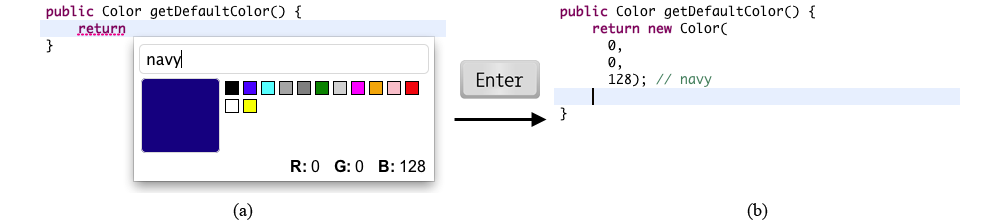
\includegraphics[width=40pc]{color_palette.png}\end{center}
% \caption{(a) An example code completion palette associated with the \texttt{Color} class. (b) The elaboration generated by this palette.}
% \label{colorpalette}
% \end{figure}

% \noindent
% Software developers make heavy use of the code completion feature of type-aware source code editors  \cite{murphy_how_2006}. Code completion typically takes the form of a floating menu containing  contextually-relevant variables, assignables, fields, methods, types and other code snippets. When an item in this menu is selected, code is inserted immediately, without further input from the developer.  By navigating and selecting from this menu, developers are able to avoid many common spelling and logic errors, eliminate unnecessary keystrokes and explore unfamiliar APIs without incurring the mental overhead associated with switching to an external documentation tool. These features have also found their way into proof assistants, e.g. the Emacs mode for Agda, where forms of code completion simplify the construction of proofs.
% % The way code completion menus brought documentation systems into the editor, active code completion interfaces bring external tools into the editor.

% %Several refinements and additions to the code completion menu have previously been suggested in the literature. These have focused on leveraging additional sources of information, such as databases of usage history \cite{robbes_how_2008}\cite{HouPletcher2011}, inheritance information \cite{HouPletcher2011}, API-specific information \cite{HouPletcher2011}\cite{Lee+2008}, partial abbreviations \cite{Han+2009}, examples extracted from code repositories \cite{bruch_learning_2009}\cite{Brandt+2010} and crowdsourced information \cite{mooty_calcite:_2010}\cite{SnipMatch}, to increase the relevance and sophistication of the featured menu items. As with the standard form of code completion, many of these sources of data can also be utilized via external tools (e.g. Calcite \cite{mooty_calcite:_2010} uses information that could already be accessed using the Jadeite \cite{conf/vl/StylosFYM09} tool). Empirical evidence presented in these studies, however, suggests that directly integrating these kinds of tools into the editor is particularly effective. For example, users of the Calcite tool completed 40\% more tasks in a lab study (unfortunately, a Jadeite control group was not included.)

% Contemporary code completion systems are difficult to extend because a fixed strategy determines the completions that are available. Library providers cannot directly specify specialized code generation logic or provide more interactive forms of assistance. 


% \begin{contribution}[Active Code Completion]
% We introduce a technique called {\it active code completion} that  make it possible to extend a code editor with  tycon-specific code generation interfaces, invoked via the familiar code completion command.% This technique is motivated by the evidence discussed above and further evidence provided in this paper that developers prefer, and make more effective use of, tools that do not require leaving the immediate editing environment.

%  We discuss active code completion in the context of object construction in Java rather than Wyvern or ML because 1) type-aware editors for Java are better developed than those for other languages; 2) we wished to do empirical studies; and (3) because Java already provides a way to associate metadata with classes. The techniques in this section apply equally well to type-aware editors for any system with a similar set of basic mechanisms. 

% For example, consider the following Java code fragment:
% \begin{lstlisting}[language=Java,numbers=none]
%   public Color getDefaultColor() {
%       return _
% \end{lstlisting}
% If the developer invokes the code completion command at the indicated cursor position (\li{_}), the editor  looks  for a {\it palette definition} associated with the {\it type} that the expression being entered is being analyzed against, which in this case is  \verb|Color| (due to the return type annotation on the method). If an associated palette is found, a menu item briefly describing this palette is added to the standard code completion menu. When selected, the corresponding palette is shown, replacing the standard code completion menu. Figure \ref{colorpalette}(a) gives an example of a simple palette that may be associated with the \verb|Color| class\footnote{A video demonstrating this process is available at \url{http://www.cs.cmu.edu/~NatProg/graphite.html}.}. 

% The developer can interact with such palettes to provide parameters and other information related to their intent, and receive immediate feedback about the effect these choices will have on the behavior of the value being constructed. When this interaction is complete, the palette produces an elaboration for insertion at the cursor, of the type (here, class) that the palette was associated with (Figure \ref{colorpalette}(b)).

% This is, in essence, an edit-time variant of the mechanism used in Wyvern to support type-specific syntax. As in Sec. \ref{sec:syntax}, we associate a palette with a declared tycon by providing metadata, here in the form of a class annotation. For example, we might write:
% \begin{lstlisting}[language=Java]
% @GraphitePalette(url="http://cs.cmu.edu/~comar/color-palette.html")
% class Color { ... }
% \end{lstlisting}
% Were a type-aware editor for Wyvern written, it might instead use metadata:
% \begin{lstlisting}
% objtype Color
%   ...
%   metadata : HasPalette = new
%     val palette_url = <SURLhttp://cs.cmu.edu/~comar/color-palette.htmlEURL>
% \end{lstlisting}
% \end{contribution}

% \begin{contribution}[Preliminary Developer Survey] 
% We sought to address the following questions before designing and implementing our active code completion system:

% \begin{itemize}
% \item What {\it specific} use cases exist for this form of active code completion in a professional development setting? 
% \item What {\it general} criteria are common to types that would and would not benefit from an associated palette?
% \item What are some relevant usability and design criteria for palettes designed to address such use cases?
% \item What capabilities must the underlying active code completion system provide to enable these use cases and user interface designs?
% \end{itemize}

% To help us answer these design questions, we conducted a survey of 473 professional developers. Their responses, along with information gathered from informal interviews and code corpus analyses, revealed a number of non-trivial functional requirements for palette interfaces as well as the underlying active code completion architecture. The primary concerns relevant to this thesis are:
% \begin{itemize}
% \item The palette mechanism should not be tied to a specific editor implementation.% We achieve this by using a URL-based scheme for referring to palettes, which are implemented as webpages. Thus, they can be embedded into any editor using standard techniques for embedding browsers into GUIs.
% \item The palette mechanism should not be able to arbitrarily access the surrounding source code. %By using a browser, and only allowing access to highlighted strings, we avoid this problem.
% \item We provide a mechanism by which users can associate palettes with types externally. This could cause conflicts with palettes that the type defines itself. %To resolve this, we give users a choice whenever such situations occur by inserting all relevant palettes into the code completion menu.
% \end{itemize}

% Participants also suggested a large number of use cases, demonstrating the broad applicability of this technique. We organized these into several broad categories. 
% \end{contribution}

% \begin{contribution}[Design and Implementation of Graphite]
% Next, we developed Graphite, an Eclipse plug-in that implements the active code completion architecture for the Java programming language, allowing Java library developers to associate custom palettes with their own classes. We describe several design choices that we made to satisfy the requirements discovered in our preliminary investigations and examine trade-offs. 
% \end{contribution}

% \begin{contribution}[Graphite Pilot Study]
% Finally, we conducted a pilot lab study with a more complex palette, implemented using Graphite, that assists developers as they write regular expressions. The study provides specific evidence in support of the broader claim that highly-specialized tools that are integrated directly with the editing environment are  useful. We conclude that active code completion systems like Graphite are useful because they make developing, deploying and discovering such tools fundamentally simpler.
% \end{contribution}


% \subsection{Timeline}
% This work has been published at ICSE 2012 \cite{Omar:2012:ACC:2337223.2337324} and we do not anticipate further work.% The main remaining tasks have to do with specifying it in terms of the bidirectional typing mechanisms in Sec. 3 more directly, rather than informally as in our paper. We plan to do this when writing the dissertation. %There are also some pieces of related work that have been published since this paper was accepted that we need to review. 


% % Finally, in Sec. \ref{acc}, we show an example of a novel class of \textbf{editor services} that can be implemented within libraries, introducing a technique we call \emph{active code completion}. Code completion is a common editor service (found in editors like Vim and Emacs as well as in the editor components of development environments like Eclipse) that helps programmers  by providing a menu of code snippets based on the surrounding code context. This is a useful but rather generic user interface. There are a variety of tools in the literature and online that help programmers generate code snippets using alternative, more specialized user interfaces. For example, a regular expression workbench helps programmers write regular expression patterns more easily (e.g. \cite{IntelliJRegexp,_txt2re:_????}). A color chooser can be considered a specialized user interface for creating an expression of type \verb|Color|. 
% % Active code completion brings these kinds of type-specific code generation interfaces, which we call \emph{palettes}, into the editor, and allows library providers to associate them with their own type constructors. Clients discover and invoke palettes from the standard code completion menu, populated according to the expected type at the cursor (a protocol similar to the one we use for syntax extensions in Wyvern). When the interaction between the client and the palette is complete, the palette produces an elaboration based on the information received from the user (the reader may wish to skip ahead to Fig. \ref{colorpalette} in Sec. \ref{acc} for an example). Using several empirical
% % methods, including a large developer survey, we examine the expressive power of this approach and develop design criteria. We then develop an active code completion system called Graphite. 
% % %Palettes are implemented as sandboxed webpages, avoiding excessive reliance on any particular editor implementation (our initial implementation is as a very simple Eclipse extension). 
% % Using Graphite,
% % we implement a palette for working with regular expressions and conduct a small study that demonstrates usefulness.% as compared to similar externally-available tools.

% % Taken together, this work aims to demonstrate that ``actively typed'' mechanisms can be introduced into many different kinds of programming systems to increase generality without the complexities of previous approaches. We approach the problem both by building up from first principles with type-theoretic models, and by developing practical designs and providing realistic contemporary examples.  
% % %It is precisely our type-oriented approach that makes it possible to guarantee that features introduced by extension providers will be safely composable in any combination. 
% % In the future, we anticipate that this work will be unified to provide foundations for a programming system organized around a minimal, well-specified and mechanically verified core, where nearly every feature is specified and implemented in a decentralized manner.% We conclude with a brief historic discussion in Sec. \ref{conclusion}.

% %
% %This suggests that a natural place where these features can be defined is in the library containing the declaration of \verb|Pattern| itself, rather than in the language and tool implementations. An \emph{actively-typed} definition of \verb|Pattern| would thus be equipped with	 functions that described how the parser (item 1), type checker (item 2), translator (item 3) and editor (item 4) should operate when working with expressions of type \verb|Pattern|. We can abstractly denote this declaration, as it would exist within a user-defined library, as follows:
% %\begin{equation*}
% %{\sf type}~Pattern[f_{\text{editor}}]\{
% %\textbf{z}[f_{\text{resolve-z}}, f_{\text{compile-z}}], 
% %\textbf{s}[f_{\text{resolve-s}}, f_{\text{compile-s}}], 
% %\textbf{natrec}[f_{\text{resolve-rec}}, f_{\text{compile-rec}}]\}
% %\end{equation*}
% %
% %When type checking an expression like $\nats{\nats{\natz}}$, the type checker delegates to the user-provided type-level function $f_{\text{resolve-s}}$. This function would be tasked with assigning a type to expression as a whole, given information including the \emph{types} (but not necessarily the full syntax trees) of all its subexpressions, or if a type cannot be assigned, producing a specific error message. Similarly, the compiler calls the $f_{\text{compile-s}}$ function to determine a representation in the target language for the expression, checking to ensure that it is well-formed and type-correct with respect to the target type system. Finally, elements of the editor may call into the $f_{\text{editor}}$ function (or one of several such functions, more generally) to control behaviors like code completion and code prediction when an expression of type $\nat$ is being entered. 
% %
% %Note that these functions are \emph{not} to be conflated with methods or run-time functions -- they are functions written in a type-level language that are called at compile-time and edit-time to define the basic behaviors associated with the type that they are associated with.
% %
% %\subsection{Characteristics of an Actively-Typed Programming System}
% %An actively-typed programming system can be characterized by its choice of type-level language, source grammar, target language and dispatch protocols.
% %
% %\paragraph{Type-Level Language} The type-level language is the language within which the type definitions and the functions that define their behaviors are defined. This language must be constrained so that different definitions do not interfere with one another and so that desirable safety properties for the system as a whole are maintained, as we discuss below.
% %
% %\paragraph{Source Language} The source language is the language with which run-time behavior is defined. In our example above, terms like $\nats{\nats{\natz}}$ are part of the source language. In the purest case, the source language is simply a grammar; its semantics are given entirely by active type specifications.
% %
% %\paragraph{Dispatch Protocol} For each syntactic form in the source language, there is a dispatch protocol that determines which type is delegated responsibility over it, and which specific function(s) are called for each behavior the system supports. This fixed protocol makes it possible for users to predict the meaning of a construct using information local to the term, a key differentiator of this approach compared to term-rewriting systems where there can be action at a distance.
% %
% %\paragraph{Target Language} The target language is the language that the front-end compilation phase of the system targets. The limitations and constraints imposed by the target language are final, because all constructs ultimately translate into terms in the target language. In other words, active type specifications can only add additional invariants to the language; they cannot violate invariants imposed by the target language.

% %\subsection{Research Challenges}
% %The example of natural numbers given above is relatively simple, and the solution we outline remains abstract. A key challenge is then to demonstrate that this approach is able to express the behaviors of more sophisticated language constructs that span diverse problem domains, and be implemented in the context of a realistic collection of tools. The resulting system should be usable by developers who lack the expertise needed to define new language constructs themselves.
% %
% %Simultaneously, we must also demonstrate that this model is well-motivated theoretically, place it within the broader context of the theory of typed programming languages, and demonstrate that it is possible for desirable system safety properties to be maintained. In particular, we are interested in properties like:
% %
% %\begin{itemize}
% %\item Correctness of active type specifications, so that users of a library need not be forced to debug errors arising within the specifications themselves.
% %\item Correctness of translations, so that the results of translation are guaranteed to be well-typed and consistent with respect to the target language.
% %\item Termination of active type specifications, so that evaluation of the type-level functions cannot cause the compiler or editor to hang.
% %\item Composability of active type specifications, so that the behaviors defined by one type cannot interfere with those defined by another, no matter the order in which they are imported. This property is essential if we wish to place these specifications within normal libraries.
% %\end{itemize}


